%
%
% UCSD Doctoral Dissertation Template
% -----------------------------------
% https://github.com/ucsd-thesis/ucsd-thesis
%
%   Lots of information can be found on the project wiki:
%   http://code.google.com/p/ucsd-thesis/wiki/GettingStarted
%
% HELP/CONTACT:
%
%   If you need help try the ucsd-thesis google group:
%   http://groups.google.com/group/ucsd-thesis
%
%
%
%
% ----------------------------------------------------------------------
% More control of the formatting of your thesis can be achieved through
% modifications of the included LaTeX class files:
%
%   * ucsd.cls    -- Class file
%   * uct10.clo   -- Configuration files for font sizes 10pt, 11pt, 12pt
%     uct11.clo                            
%     uct12.clo
%
% ----------------------------------------------------------------------



% Setup the documentclass 
% default options: 12pt, oneside, final
%
% fonts: 10pt, 11pt, 12pt -- are valid for UCSD dissertations.
% sides: oneside, twoside -- note that two-sided theses are not accepted 
%                            by OGS.
% mode: draft, final      -- draft mode switches to single spacing, 
%                            removes hyperlinks, and places a black box
%                            at every overfull hbox (check these before
%                            submission).
% chapterheads            -- Include this if you want your chapters to read:
%                              Chapter 1
%                              Title of Chapter
%
%                            instead of
%                              1 Title of Chapter
\documentclass[12pt,chapterheads]{ucsd}



% Include all packages you need here.  
% Some standard options are suggested below.
%
% See the project wiki for information on how to use 
% these packages. Other useful packages are also listed there.
%
%   http://code.google.com/p/ucsd-thesis/wiki/GettingStarted



%% AMS PACKAGES - Chances are you will want some or all 
%    of these if writing a dissertation that includes equations.
  \usepackage{amsmath, amscd, amssymb, amsthm,mathtools}

%% MARGIN REQUIREMENTS IN TITLES - Hyphenation in a Section Title does not always respect margin settings in Latex.  To force no hyphentation, uncomment the package below.
%  \usepackage[raggedright]{titlesec} 

%% GRAPHICX - This is the standard package for 
%    including graphics for latex/pdflatex.
\usepackage{scrextend}
\usepackage{pslatex}
\usepackage{graphicx}
\usepackage{caption}
\usepackage{subcaption}

\usepackage{fullpage,hyperref,tikz-cd}
\usepackage[all]{xy}
\usepackage[normalem]{ulem}


\newtheorem{theorem}{Theorem}[section]
\newtheorem{lemma}[theorem]{Lemma}
\newtheorem{cor}[theorem]{Corollary}
\newtheorem{problem}[theorem]{Problem}
\newtheorem{algorithm}[theorem]{Algorithm}
\theoremstyle{definition}
\newtheorem{defn}[theorem]{Definition}
\newtheorem{remark}[theorem]{Remark}
\newtheorem{conj}[theorem]{Conjecture}
\newtheorem{example}[theorem]{Example}
\newtheorem{proposition}[theorem]{Proposition}

\newcommand{\FF}{\mathbb{F}}
\newcommand{\QQ}{\mathbb{Q}}
\newcommand{\RR}{\mathbb{R}}
\newcommand{\ZZ}{\mathbb{Z}}
\newcommand{\HH}{\mathbb{H}}
\newcommand{\CC}{\mathbb{C}}

\newcommand{\frakp}{\mathfrak{p}}
\newcommand{\PP}{\mathbb{P}}

\newcommand{\calM}{\mathcal{M}}
\newcommand{\calO}{\mathcal{O}}
\newcommand{\calS}{\mathcal{S}}

\newcommand{\slz}{\SL_2(\ZZ)}


\DeclareMathOperator{\coker}{coker}
\DeclareMathOperator{\End}{End}
\DeclareMathOperator{\Ext}{Ext}
\DeclareMathOperator{\GL}{GL}
\DeclareMathOperator{\SL}{SL}
\DeclareMathOperator{\Gal}{Gal}
\DeclareMathOperator{\Gr}{Gr}
\DeclareMathOperator{\Hom}{Hom}
\DeclareMathOperator{\OG}{OG}
\DeclareMathOperator{\PGL}{PGL}
\DeclareMathOperator{\Proj}{Proj}
\DeclareMathOperator{\PSL}{PSL}
\DeclareMathOperator{\SO}{SO}
\DeclareMathOperator{\SpG}{SpG}
\DeclareMathOperator{\Stab}{Stab}
\DeclareMathOperator{\Sym}{Sym}
\DeclareMathOperator{\Trace}{Trace}
%\DeclareMathOperator{\det}{det}
\DeclareMathOperator{\Div}{Div}


\newcommand{\todo}[1]{\textcolor{red}{\textbf{TODO: #1}}}

\newcommand{\Gap}{\textsc{GAP}}
\newcommand{\Magma}{\textsc{Magma}{}}
\newcommand{\SageMath}{\textsc{SageMath}}
\newcommand{\Singular}{\textsc{Singular}}

%% Links to arXiv
\newcommand{\arXiv}[3]{\href{https://arxiv.org/abs/#1}{arXiv:#1v#2} (#3)}

%% CAPTION
% This overrides some of the ugliness in ucsd.cls and
% allows the text to be double-spaced while letting figures,
% tables, and footnotes to be single-spaced--all OGS requirements.
% NOTE: Must appear after graphics and ams math
\makeatletter
\gdef\@ptsize{2}% 12pt documents
\let\@currsize\normalsize
\makeatother
\usepackage{setspace}
\doublespace
\usepackage[font=small, width=0.9\textwidth]{caption}

\usepackage[capposition=bottom]{floatrow} %force captions below figure per OGS requirement

%% SUBFIG - Use this to place multiple images in a
%    single figure.  Subfig will handle placement and
%    proper captioning (e.g. Figure 1.2(a))
% \usepackage{subfig}

%% TIMES FONT - replacements for Computer Modern
%%   This package will replace the default font with a
%%   Times-Roman font with math support.
 \usepackage[T1]{fontenc}
 \usepackage{mathptmx}



%% INDEX
%   Uncomment the following two lines to create an index: 
% \usepackage{makeidx}
% \makeindex
%   You will need to uncomment the \printindex line near the
%   bibliography to display the index.  Use the command
% \index{keyword} 
%   within the text to create an entry in the index for keyword.
%   To compile a LaTeX document with an index the 'makeindex'
%   command will need to be run.  See the wiki for more details.

%% HYPERLINKS
%   To create a PDF with hyperlinks, you need to include the hyperref package.
%   THIS HAS TO BE THE LAST PACKAGE INCLUDED!
%   Note that the options plainpages=false and pdfpagelabels exist
%   to fix indexing associated with having both (ii) and (2) as pages.
%   Also, all links must be black according to OGS.
%   See: http://www.tex.ac.uk/cgi-bin/texfaq2html?label=hyperdupdest
%   Note: This may not work correctly with all DVI viewers (i.e. Yap breaks).
%   NOTE: hyperref will NOT work in draft mode, as noted above.
% \usepackage[colorlinks=true, pdfstartview=FitV, 
%             linkcolor=black, citecolor=black, 
%             urlcolor=black, plainpages=false,
%             pdfpagelabels]{hyperref}
% \hypersetup{ pdfauthor = {Your Name Here}, 
%              pdftitle = {The Title of The Dissertation}, 
%              pdfkeywords = {Keywords for Searching}, 
%              pdfcreator = {pdfLaTeX with hyperref package}, 
%              pdfproducer = {pdfLaTeX} }
% \urlstyle{same}
% \usepackage{bookmark}


%% CITATIONS
% Sets citation format
% and fixes up citations madness
\usepackage{microtype}  % avoids citations that hang into the margin


%% FOOTNOTE-MAGIC
% Enables footnotes in tables, re-referencing the same footnote multiple times.
\usepackage{footnote}
\makesavenoteenv{tabular}
\makesavenoteenv{table}


%% TABLE FORMATTING MADNESS
% Enable all sorts of fun table tricks
\usepackage{rotating}  % Enables the sideways environment (NCPW)
\usepackage{array}  % Enables "m" tabular environment http://ctan.org/pkg/array
\usepackage{booktabs}  % Enables \toprule  http://ctan.org/pkg/array



\begin{document}

%% FRONT MATTER
%
%  All of the front matter.
%  This includes the title, degree, dedication, vita, abstract, etc..
%  Modify the file template_frontmatter.tex to change these pages.
%
%
% UCSD Doctoral Dissertation Template
% -----------------------------------
% http://ucsd-thesis.googlecode.com
%
%


%% REQUIRED FIELDS -- Replace with the values appropriate to you

% No symbols, formulas, superscripts, or Greek letters are allowed
% in your title.
\title{$p$-adic Integration on Modular Curves and Code-Based Cryptography}

\author{Jun Bo Lau}
\degreeyear{\the\year}

% Master's Degree theses will NOT be formatted properly with this file.
\degreetitle{Doctor of Philosophy}

\field{Mathematics}

\chair{Professor Kiran Kedlaya}
% Uncomment the next line iff you have a Co-Chair
% \cochair{Professor Cochair Semimaster}
%
% Or, uncomment the next line iff you have two equal Co-Chairs.
%\cochairs{Professor Chair Masterish}{Professor Chair Masterish}

%  The rest of the committee members  must be alphabetized by last name.
\othermembers{
Professor Russell Impagliazzo\\
Professor Jonathan Novak\\
Professor Cristian Popescu\\
Professor Claus Sorensen
}
\numberofmembers{5} % |chair| + |cochair| + |othermembers|


%% START THE FRONTMATTER
%
\begin{frontmatter}

%% TITLE PAGES
%
%  This command generates the title, copyright, and signature pages.
%
\makefrontmatter

%% DEDICATION
%
%  You have three choices here:
%    1. Use the ``dedication'' environment.
%       Put in the text you want, and everything will be formated for
%       you. You'll get a perfectly respectable dedication page.
%
%
%    2. Use the ``mydedication'' environment.  If you don't like the
%       formatting of option 1, use this environment and format things
%       however you wish.
%
%    3. If you don't want a dedication, it's not required.
%
%
%\begin{dedication}
%  To two, the loneliest number since the number one.
%\end{dedication}


% \begin{mydedication} % You are responsible for formatting here.
%   \vspace{1in}
%   \begin{flushleft}
% 	To me.
%   \end{flushleft}
%
%   \vspace{2in}
%   \begin{center}
% 	And you.
%   \end{center}
%
%   \vspace{2in}
%   \begin{flushright}
% 	Which equals us.
%   \end{flushright}
% \end{mydedication}



%% EPIGRAPH
%
%  The same choices that applied to the dedication apply here.
%
\begin{epigraph} % The style file will position the text for you.
  \emph{A careful quotation\\
  conveys brilliance.}\\
  ---Smarty Pants
\end{epigraph}

% \begin{myepigraph} % You position the text yourself.
%   \vfil
%   \begin{center}
%     {\bf Think! It ain't illegal yet.}
%
% 	\emph{---George Clinton}
%   \end{center}
% \end{myepigraph}


%% SETUP THE TABLE OF CONTENTS
%
\tableofcontents
%\listoffigures  % Comment if you don't have any figures
%\listoftables   % Comment if you don't have any tables



%% ACKNOWLEDGEMENTS
%
%  While technically optional, you probably have someone to thank.
%  Also, a paragraph acknowledging all coauthors and publishers (if
%  you have any) is required in the acknowledgements page and as the
%  last paragraph of text at the end of each respective chapter. See
%  the OGS Formatting Manual for more information.
%
\begin{acknowledgements}
 Thanks to whoever deserves credit for Blacks Beach, Porters Pub, and
 every coffee shop in San Diego.

 Thanks also to hottubs.
\end{acknowledgements}


%% VITA
%
%  A brief vita is required in a doctoral thesis. See the OGS
%  Formatting Manual for more information.
%
\begin{vitapage}
\begin{vita}
  \item[2017] M.Math University of Warwick, U.K.
  \item[2017-2023] Graduate Teaching Assistant, University of California, San Diego
  \item[2023] Ph.~D. in Mathematics, University of California, San Diego
\end{vita}
\end{vitapage}


%% ABSTRACT
%
%  Doctoral dissertation abstracts should not exceed 350 words.
%   The abstract may continue to a second page if necessary.
%
\begin{abstract}
In this dissertation, we study two problems arising from arithmetic geometry.

Falting's theorem states that there are only finitely many rational points on curves of genus greater than 1. However, an explicit determination of all such points on a curve remains a hard problem. There are various approaches to computing rational points on higher genus curves and we use Coleman's theory of $p$-adic line integrals to study a particular class of curves with rich arithmetic origins, namely, the modular curves. In join work with Chen and Kedlaya, we implement a new algorithm that does not use the models of the modular curves and illustrate this method through the computation of several examples.

On the other hand, in anticipation of the development of powerful quantum computers in the next few decades, we study cryptosystems that rely on the hardness of certain number theoretical problems. In particular, we investigate BIKE, a cryptosystem presented as one of the candidates for the National Institute of Standards and Technology Post-Quantum Cryptography Standardization Process. We identified several factors that affect the security of the code-based cryptosystem as a potential quantum-attack-resistant candidate for real world applications through extensive simulations.


\end{abstract}


\end{frontmatter}






%% DISSERTATION

% A common strategy here is to include files for each of the chapters. I.e.,
% Place the chapters is separate files: 
%   chapter1.tex, chapter2.tex
% Then use the commands:
%   \include{chapter1}
%   \include{chapter2}
%
% Of course, if you prefer, you can just start with
%   \chapter{My First Chapter Name}
% and start typing away.  

%%%%%%%%%%%%%%%%%%%%%% \include{sample_unused}

\part{Coleman Integration on Modular Curves}
\chapter{Preliminaries}

All curves in this paper are smooth, projective and geometrically irreducible with good reduction at a prime $p$.

\section{Introduction}

Some of the oldest questions in number theory can be reformulated in modern terms: given a finite list of polynomials, what are the integer or rational solutions to this set of equations? In fact, these solutions can be viewed as integer or rational solutions of geometric objects -- curves, surfaces or higher dimensional objects.

In this project, we focus on the case of curves. A remarkable result, formulated by Mordell in 1922 and proved by Faltings in 1983, states that for curves of higher genus, there are only finitely many rational points on them. 

\begin{theorem}{(Mordell's conjecture/ Faltings's theorem)} Let $X/\QQ$ be a curve of genus $g \geq 2$, then the set of rational points $X(\QQ)$ is finite.
\end{theorem}

However, Faltings's proofs are not effective, i.e., there is no way of explicitly determining the complete set of rational points on the curve. Before Faltings, Chabauty developed a method in this direction with the condition that if the rank of the Jacobian of the curve is strictly less than the genus, then one could compute this set of points. In \cite{Coleman2,Coleman3} Coleman defined $p$-adic line integrals and re-interpreted Chabauty's method to explicitly compute the set of rational points. These Coleman integrals provide an effective method to problems in arithmetic geometry, including but not limited to, torsion points on Jacobians of curves ( Manin-Mumford conjecture), $p$-adic heights on curves, $p$-adic polylogarithms, Mordell conjecture (rational points), etc. In \cite{BD1,BD2}, Balakrishnan and Dogra developed quadratic Chabauty as a computational tool to study the set of rational points as long as the curve satisfies a certain quadratic Chabauty bound, involving the rank of the Jacobian, genus and N\'{e}ron-Severi rank of the Jacobian.

There are several approaches to numerically compute these Coleman integrals. Wetherell \cite{wetherell} combined the certan properties of Coleman integrals and the arithmetic of the Jacobian to compute $\int_D \omega$, where $D$ is a divisor in the Picard group and $\omega$ is a holomorphic differential on the curve. The next approach relies on computing the Frobenius action in $p$-adic cohomology following Dwork's principle of analytic continuation along the Frobenius \cite{BBK10,Tui16,Tui17,BT_coleman}. However, both of these approaches have their shortcomings -- Wetherell's method requires an explicit divisor in order to reduce the computation to a power series integration (``tiny integrals") and the second method requires an explicit equation of the curves as input.

We turn our attention to computing Coleman integrals on modular curves. The set of rational points on modular curves has special arithmetic meaning. For instance, the set of rational points $X_0(N)(\QQ)$ correspond to the torsion points of elliptic curves (Mazur's theorem). Another motivation to study modular curves comes from Serre's Uniformity Conjecture. Let $E$ be an elliptic curve defined over $K$. The group of $p$-torsion points $E[p](\bar{K})$ is isomorphic to $(\ZZ/p\ZZ)^2$ and is acted upon by the absolute Galois group $\Gal(\bar{K}/K)$, giving rise to a representation $\rho_ {p,E}: \Gal(\bar{K}/K) \rightarrow \GL_2(\FF_p)$. In \cite{serre72}, Serre proved the following:

\begin{theorem}
    Suppose that $E$ does not have complex multiplication. Then there exists a number $N(E)$ such that $\rho_{p,E}$ is surjective for all $p > N(E)$.
\end{theorem}

In the same paper, he posed the following question:

\begin{conj}{(Serre's Uniformity Conjecture)}
Given a number field $K$, then there exist a constant $N_K>0$ such that for any elliptic curve $E$ defined over $K$ without complex multiplication, the corresponding Galois representation $\rho_{p,E}$ is surjective for all primes $p > N_K$.
\end{conj}

Since modular curves parametrise elliptic curves with torsion data, this can be formulated in terms of rational points on modular curves:

\begin{conj}{(Serre's Uniformity Conjecture)}
    Let $H \leq \GL_2(\FF_p)$ be a proper subgroup such that the determinant map $\det: H \rightarrow \FF_p^\times$ is surjective, then there exist a constant $N_K>0$ such that for any prime $p> N_K$, the associated modular curve $X_H(p)$ has $K$-rational points coming only from cusps and elliptic curves with complex multiplication.
\end{conj}




If $\rho_{p,E}$ is not surjective, the image lies inside some maximal proper subgroup of $\GL_2(\FF_p)$. Therefore, one could prove the conjecture by showing that for $p$ large enough, the image of $\rho_{p,E}$ does not lie in any maximal subgroup. The classification of maximal subgroups of $\GL_2(\FF_p)$ is known, originally due to \cite{dickson}:

\begin{theorem}
    Let $H \leq \GL_2(\ZZ/p\ZZ)$ not containing $\SL_2(\ZZ/p\ZZ)$. Up to conjugacy, $H$ is one of the following:
    \begin{itemize}
        \item (Borel) $H \subseteq B_0(p) = \{ \begin{psmallmatrix} \ast \ \ast \\ 0 \ \ast \end{psmallmatrix} \}$ 
        \item (Normaliser of split Cartan) $H \subseteq N_s^+(p) = \{ \begin{psmallmatrix} \alpha \ 0 \\ 0 \ \beta \end{psmallmatrix}, \begin{psmallmatrix} 0 \ \alpha \\ \beta \ 0 \end{psmallmatrix}: \alpha,\beta \in \FF_p^\times \}$ 
        \item (Normaliser of non-split Cartan) $H \subseteq N_s^+(p) = \{ \begin{psmallmatrix} \alpha \ 0 \\ 0 \ \alpha^p \end{psmallmatrix}, \begin{psmallmatrix} 0 \ \alpha \\ \alpha^p \ 0 \end{psmallmatrix}: \alpha \in \FF_{p^2}^\times \}$ 
        \item (Exceptional) The image of $H$ in $\PGL_2(\FF_p)$ is isomorphic to $A_4,S_4$ or $A_5$.
    \end{itemize}
\end{theorem}

Most of the cases have been resolved \cite{borel,BP1,BP2,serre72}, except for the normaliser of non-split Cartan. There has been some progress using quadratic Chabauty to find the rational points of the modular curve corresponding to the nonsplit Cartan of level 13 \cite{cursed-curve} and level 17 \cite{BDMTV}.

Since most modular curves satisfy the quadratic Chabauty bound \cite{Siksek}, we provide a model-free algorithm to compute Coleman integrals on modular curves arising  arising from Serre's Uniformity Conjecture.

\section{Background}

\subsection{Modular forms}

In this section, we give a brief introduction of modular forms, following \cite{Shurman}.

Let $\HH := \{ \tau \in \CC: Im(\tau) > 0 \}$ be the upper half complex plane. The special linear group $\SL_2(\ZZ)$ acts on $\HH$ via fractional linear transformations:

\[
\gamma \cdot \tau = \frac{a\tau + b}{c \tau + d}
\] 

where $\gamma = \begin{psmallmatrix} a & b \\ c & d \end{psmallmatrix}, \tau \in \HH$. 

\begin{defn}
Let $f: \HH \rightarrow \CC$ be a function and $k \in \ZZ$. 

\begin{itemize}
    \item The \textit{automorphy factor} is a function \begin{align*}j: \GL_2^+(\RR) \times \HH &\rightarrow \CC \\ (\gamma,z) &\mapsto cz+d \end{align*}
    where $\gamma = \begin{psmallmatrix} a & b \\ c & d \end{psmallmatrix}$.
    \item The \textit{weight-$k$ slash operator} is defined as 
    \begin{align*}
( \ \cdot \ )|_k (\ \cdot \ ): \Hom(\HH,\CC) \times \GL_2^+(\RR) &\rightarrow \Hom(\HH,\CC) \\
(f(z),\gamma) &\mapsto (f|_k \gamma)(z) := (\det \gamma)^{k-1} j(\gamma,z)^{-k} f(\gamma \cdot z).
    \end{align*}
    \end{itemize}
\end{defn}

The automorphy factory satisfies a cocycle relation $j(\gamma_1\gamma2,z) = j(\gamma_1,\gamma_2 z)j(\gamma_2,z)$ which implies that $\GL_2^+(\RR)$ acts on $\Hom(\HH,\CC)$ via $f|_k\gamma_1\gamma_2 = (f|_k\gamma_1)|_k\gamma_2$.

Consider the projection map $\pi: \SL_2(\ZZ) \rightarrow \SL_2(\ZZ/N\ZZ)$. We define congruence subgroups in the following way.

\begin{example}\label{example:1_congsgp}
Here are some common examples of preimages of $\pi$:

\begin{itemize}
    \item $\Gamma(N) = \pi^{-1} (\begin{psmallmatrix}
        1 & 0 \\ 0 & 1
    \end{psmallmatrix}) = \{ \begin{psmallmatrix}
        a & b \\ c & d 
    \end{psmallmatrix} \in \SL_2(\ZZ): \begin{psmallmatrix}
        a & b \\ c & d 
    \end{psmallmatrix} \equiv \begin{psmallmatrix}
        1 & 0 \\ 0 & 1 
    \end{psmallmatrix} \pmod{N}\}$.
    \item $\Gamma_1(N) = \pi^{-1} (\{\begin{psmallmatrix}
        1 & \ast \\ 0 & 1
    \end{psmallmatrix}\}) = \{ \begin{psmallmatrix}
        a & b \\ c & d 
    \end{psmallmatrix} \in \SL_2(\ZZ): \begin{psmallmatrix}
        a & b \\ c & d 
    \end{psmallmatrix} \equiv \begin{psmallmatrix}
        1 & \ast \\ 0 & 1 
    \end{psmallmatrix} \pmod{N}\}$.
    \item $\Gamma_0(N) = \pi^{-1} (\{\begin{psmallmatrix}
        \ast & \ast \\ 0 & \ast
    \end{psmallmatrix}\}) = \{ \begin{psmallmatrix}
        a & b \\ c & d 
    \end{psmallmatrix} \in \SL_2(\ZZ): \begin{psmallmatrix}
        a & b \\ c & d 
    \end{psmallmatrix} \equiv \begin{psmallmatrix}
        \ast & \ast \\ 0 & \ast 
    \end{psmallmatrix} \pmod{N}\}$.
\end{itemize}
\end{example}

\begin{defn}
$\Gamma \leq \SL_2(\ZZ)$ is a \textit{congruence subgroup} if there exists an integer $N \geq 1$ such that $\Gamma(N) \leq \Gamma$. The minimal such $N$ is called the \textit{level} of $\Gamma$.

It follows immediately that congruence subgroups of $\SL_2(\ZZ)$ have finite index and correspond to subgroups of $\SL_2(\ZZ/N\ZZ)$. The above examples are all congruence subgroups of level $N$.
\end{defn}

\begin{defn}
    Let $\Gamma \leq \SL_2(\ZZ)$ be a congruence subgroup of level $N$, $k \geq 0$ an integer. We say a function $f: \HH \rightarrow \CC$ is a \textit{modular form of weight $k$ with level $\Gamma$} if

    \begin{enumerate}
        \item $f$ is holomorphic,
        \item $f$ is weight-$k$ invariant under $\Gamma$, i.e., $f|_k\gamma = f$ for all $\gamma \in \Gamma$,
        \item $f|_k\alpha $ is holomorphic at $\infty$ for all $\alpha \in \SL_2(\ZZ)$, i.e., $(f|_k \alpha )(z)$ is bounded as $z \rightarrow i\infty$.
    \end{enumerate}

    If, in addition, $f|_k \alpha$ vanishes at infinity for all $\alpha \in \SL_2(\ZZ)$, we say that $f$ is a \textit{cusp form}. We denote the set of weight-$k$ modular forms with respect to $\Gamma$ (resp. cusp forms) as $\mathcal{M}_k(\Gamma)$ (resp. $\mathcal{S}_k(\Gamma)$).
\end{defn}

Suppose $f$ is a modular form of weight $k$ with level $\Gamma$. Since $\Gamma$ is a congruence subgroup, $\begin{psmallmatrix}
    1 & h \\ 0 & 1
\end{psmallmatrix} \in \Gamma$ for some minimal integer $h\geq 1$, this integer is the \textit{width} of the cusp $\infty$. Since a modular form satisfies $f|_k \gamma = f$ for $\gamma \in \Gamma$, we have $(f|_k \begin{psmallmatrix}
    1 & h \\ 0 & 1
\end{psmallmatrix})(z) = f(z+h) = f(z) $, so $f(z)$ is $h\ZZ$-periodic and admits a Fourier expansion $f(\tau) = \sum_{n=0}^\infty a_n q_{h}^n$ where $q_h = \exp(2\pi i\tau / h)$. The third condition of modular forms implies that the Fourier expansion begins at index $0$ and cusp forms satisfy $a_0 = 0$.

\begin{example}
Let $G_k(\tau) = \sum_{(c,d) \not = (0,0)} 1/(c\tau + d)^k$. This is a modular form of weight $k$ for $\SL_2(\ZZ)$ called \textit{Eisenstein series}. 

    The \textit{$j$-invariant} is a modular form of weight $0$, i.e., a modular function and an element of $\CC(X(\SL_2(\ZZ)))$, with $q$-expansion:

    \begin{align*}
        j: \HH \rightarrow \CC, j(\tau) = 1728 \frac{(60 G_4(\tau))^3}{(60 G_4(\tau))^3 - 27 (140 G_6(\tau))^2} = \frac{1}{q} + 744 + 196884q + \ldots.
    \end{align*}
\end{example}

It is a standard result that $\mathcal{M}_k(\Gamma) \supseteq \mathcal{S}_k(\Gamma)$ are finite dimensional complex vector spaces. Modular forms and modular curves are related by the fact that there is an isomorphism between the space of weight $2$ cusp forms and the space of holomorphic differentials on the modular curve $X(\Gamma)$. 

\begin{align*}
\mathcal{S}_2(\Gamma) &\xrightarrow{\cong} H^0(X(\Gamma),\Omega^1) \\
f(\tau) &\mapsto f(\tau) d\tau.
\end{align*}
%
\subsection{Modular curves}
In this section, we define our object of study. Modular curves have rich structures as Riemann surfaces, algebraic curves and moduli spaces of elliptic curves (with some torsion information). We frequently use properties from various perspectives interchangeably.

\subsubsection{As Riemann surfaces}
Let $\Gamma \leq \SL_2(\ZZ)$ be a subgroup of finite index. $\HH$ inherits the Euclidean topology from $\CC$ and so $Y(\Gamma) := \Gamma \backslash \HH$ carries the quotient topology that is Hausdorff. $Y(\Gamma)$ can be compactified by adjoining cusps, which are orbits of $\PP^1(\QQ)$ under the action of $\Gamma$. The resulting quotient space $X(\Gamma) := \Gamma \backslash \HH^*$ where $\HH^* := \HH \cup \PP^1(\QQ)$ is called the modular curve associated to $\Gamma$. One could further show that by considering elliptic points and cusps, one can choose suitable charts, therefore giving $Y(\Gamma)$ and $X(\Gamma)$ the structure of Riemann surface.

This approach allows us to use techniques from Riemann surfaces, e.g., genus/ramification theory, Riemann-Hurwitz formula, Riemann-Roch, etc. to study modular curves.

\subsubsection{As algebraic curves}

For a finite index subgroup $\Gamma \leq \SL_2(\ZZ)$. The associated modular curve $X(\Gamma)$ has the structure of a compact Riemann surface. Compact Riemann surfaces and complex algebraic curves are equivalent notions \cite{forster}. Note that we are also considering modular curves where the determinant map on the subgroup $H \leq \GL_2(\ZZ/N\ZZ)$ is surjective. By Theorem 7.6.3 in \cite{Shurman}, these algebraic curves are in fact defined over $\QQ$. We have a Galois-theoretic correspondence between curves and their function fields:

\begin{theorem}{(Curves-Fields Correspondence)} For any field $k$, there is a bijection:

\begin{align*}
\{\text{$C/k$ smooth projective algebraic curves}\}/\cong &\leftrightarrow \{\text{$K/k$ function field extensions over $k$}\}/\sim \\
C &\mapsto k(C)
\end{align*}

Furthermore, this is contravariant: a nonconstant morphism from  algebraic curves $C$ to $C'$ over $k$ corresponds to a field morphism from $k(C')$ to $k(C)$.

\end{theorem}

The above theorem allows us to work with simpler objects, i.e., we can replace curves and their morphisms by fields and field injections. In particular, the function field of the modular curve $X(\Gamma)$ consists of modular functions of weight $0$ and level $\Gamma$. 

\subsubsection{As moduli spaces of elliptic curves}

For each $\tau \in \HH$, one could associate it with a lattice $\Lambda_\tau := \ZZ + \tau \cdot \ZZ \subseteq \CC$. The resulting quotient space $\CC/\Lambda_\tau$ is a compact Riemann surface of genus $1$, an elliptic curve. Conversely, for any elliptic curve, as a genus 1 compact Riemann surface, the homology group of the elliptic curve $H_1(E,\ZZ)$ is generated by two loops, $\gamma_1, \gamma_2$. For an invariant differential $\omega$ of the elliptic curve, we can construct the lattice generated by the periods $\Lambda_E = (\int_{\gamma_1} \omega) \cdot \ZZ + (\int_{\gamma_2} \omega) \cdot \ZZ$. This can be renormalised so that $\Lambda_E = \ZZ + \tau \cdot \ZZ$ with $\tau = (\int_{\gamma_1} \omega) /(\int_{\gamma_2} \omega) \in \HH$. In particular the points on $\HH$ correspond to elliptic curves.

For $\Gamma \leq \SL_2(\ZZ)$, the modular curve $X(\Gamma)(\bar{\QQ})$ parametrise elliptic curves with some torsion data, i.e., a pair $(E, \phi)$ where $E$ is an elliptic curve defined over $\bar{\QQ}$ and $\phi$ is an isomorphism of its $N$-torsion points $\phi: E[N] \rightarrow (\ZZ/N\ZZ)^2$. Furthermore, there is an action of the absolute Galois group $Gal(\bar{\QQ}/\QQ)$ on $(E,\phi)$ and we say that $(E,\phi)$ is a $\QQ$-rational point if it is invariant under the action. We can view points on modular curves as elliptic curves with certain torsion structures which allows us to apply properties of elliptic curves to study the rational points on $X(\Gamma)$.

\begin{example}
Let $H \leq \GL_2(\ZZ/N\ZZ)$ be a subgroup such that
\begin{itemize}
    \item $-I \in H$,
    \item the determinant map $\det: H \rightarrow (\ZZ/N\ZZ)^\times$ is surjective.
\end{itemize}
Then for an integer $N \geq 1$, we have the congruence subgroup $\Gamma_H(N) = \{ A \in \SL_2(\ZZ) : A \pmod{N} \in H \}$, which gives rise to the modular curves $X_H := X(\Gamma_H(N))$.

Following Example \ref{example:1_congsgp}, the corresponding modular curves parametrise:

\begin{itemize}
    \item $X(N):= X(\Gamma(N))$ consists of $(E,(P,Q))$ an elliptic curve and a pair of points generating the $N$-torsion subgroup of $E$.
    \item $X_1(N) := X(\Gamma_1(N))$ consists of $(E,Q)$ an elliptic curve and a point of order $N$.
    \item $X_0(N) := X(\Gamma_0(N))$ consists of $(E,C)$ an elliptic curve and a cyclic subgroup of order $N$.
\end{itemize}
\end{example}
%\subsection{Hecke operators}

We begin with the definition of Hecke operators as operators on spaces of modular forms. These are used in conjunction with spectral theory to show that the inner product space of modular forms contains a basis of modular forms that are eigenvectors under the Hecke operators $\{T_p\}_p$. Hecke operators are defined on modular forms and modular curves. We use both the transcendental and algebraic/geometric definitions of Hecke operators in our algorithm.

\begin{defn}
Let $\Gamma_1, \Gamma_2$ be congruence subgroups of $SL_2(\ZZ)$ and $\alpha \in GL_2^+(\QQ)$. 

\begin{itemize}
    \item We define the \textit{double coset} $\Gamma_1 \alpha \Gamma_2$ as the set 

\[
\Gamma_1 \alpha \Gamma_2 := \{\gamma_1 \alpha \gamma_2 : \gamma_1 \in \Gamma_1, \gamma_2 \in \Gamma_2\}
\]
\item This gives rise to the \textit{double coset operators}:

\begin{align*} \label{eq:hecke_formula}
(\ \cdot \ )|_k [\Gamma_1 \alpha \Gamma_2] : \mathcal{M}_k(\Gamma_1) &\rightarrow \mathcal{M}_k(\Gamma_2) \\
f(\tau) &\mapsto f|_k \Gamma_1 \alpha \Gamma_2 := \sum_i f|_k \beta_i
\end{align*}

where $\Gamma_1 \alpha \Gamma_2 = \bigcup_i \Gamma_1 \beta_i$ is a (finite) disjoint coset decomposition that does not depend on the choice of decomposition. This map restricts to an operator on the space of cusp forms $(\ \cdot \ )|_k [\Gamma_1 \alpha \Gamma_2] : \mathcal{S}_k(\Gamma_1) \rightarrow \mathcal{S}_k(\Gamma_2)$.
\end{itemize}
\end{defn}

We follow the approach \cite{Assaf2020} to define Hecke operators.

\begin{defn}
Fix a congruence subgroup $\Gamma$ with $\bar{\Gamma} \leq SL_2(\ZZ/N\ZZ)$.
Let $\alpha \in M_2(\ZZ)$ such that $\det (\alpha) \in \det (\bar{\Gamma})$ and $\alpha \pmod{N} \in \bar{\Gamma}$. We define the Hecke operator as

\[
T_p = T_\alpha = ( \ \cdot \ )|_k [\Gamma \alpha \Gamma]
\]
\end{defn}

\begin{example} (\cite{Shurman} Prop. 5.2.1)
The theory of Hecke operators can be made explicit for certain congruence subgroups. The Hecke operator $T_p = [ \Gamma_1(N) \begin{psmallmatrix} 1 & 0 \\ 0 & p \end{psmallmatrix} \Gamma_1(N)]_k $ on $\mathcal{M}_k(\Gamma_1(N))$ has the following formulae:

\[T_p f =
\begin{cases}
\sum_{i = 0}^{p-1} f|_k \begin{psmallmatrix}
    1 & j \\ 0 & p \end{psmallmatrix}, & \text{if $p | N$,} \\
\sum_{i = 0}^{p-1} f|_k \begin{psmallmatrix}
    1 & j \\ 0 & p \end{psmallmatrix} + f|_k (\begin{psmallmatrix} m & n \\ N & p \end{psmallmatrix} \begin{psmallmatrix}
        p & 0 \\ 0 & 1
    \end{psmallmatrix}), & \text{if $p\not | N$, where $mp - nN = 1$.} \\
\end{cases} 
\]
\end{example}

We summarise a well-known result from the theory of Hecke operators to show that there is a basis of cusp forms which are eigenvectors of the Hecke operators \cite{Shurman}:

\begin{theorem}
Let $\Gamma$ be a congruence subgroup of level $N$ and $n$ an integer coprime to $N$. Then,

\begin{itemize}
\item $\mathcal{M}_k(\Gamma),\mathcal{S}_k(\Gamma)$ are inner product spaces with respect to an inner product called the \textit{Petersson inner product}.
\item The Hecke operator $T_n$ is a normal operator with respect to this inner product. There is another family of Hecke operators called the diamond operators which is also a normal operator.
\end{itemize}

Therefore, we have a commuting family of operators on a finite dimensional inner product space and the spectral theorem implies that there is an orthogonal basis of simultaneous eigenvectors formed by the cusp forms. In this case, we say that the cusp forms are \textit{Hecke eigenforms} or simply \textit{eigenforms}.
\end{theorem}

There is also an algebraic/geometric interpretation of the double coset operator as a morphism of divisor groups. For $\Gamma_1, \Gamma_2$ congruence subgroups, $\alpha \in GL_2^+(\QQ) $, $\Gamma_3 := \alpha^{-1} \Gamma_1 \alpha \cap \Gamma_2$ and $\Gamma_3' := \alpha \Gamma_3 \alpha^{-1}$. Since points on the modular curve $X(\Gamma)$ have the form $\Gamma \tau$, we have a diagram at the level of groups which induces a diagram on modular curves:


\begin{align*}
\Gamma_2 \hookleftarrow \Gamma_3 \xrightarrow{\cong} \Gamma_3' \hookrightarrow \Gamma_1 \\
X_2 \xleftarrow{\pi_2} X_3 \xrightarrow{\cong} X_3' \xrightarrow{\pi_1} X_1
\end{align*}

Suppose $\Gamma_3 / \Gamma_2 = \bigcup_j \Gamma_3 \gamma_{2,j}$ and $\beta_j = \alpha \gamma_{2,j}$. Then the double coset operator induces a map on the divisor groups  after $\ZZ$-linear extension:

\begin{align*}
    \Div(X_2) &\rightarrow \Div(X_1) \\
    \Gamma_2 \tau &\mapsto \sum_j \Gamma_1 \beta_j \tau
\end{align*}

Specialising to the case of Hecke operator, we obtain a similar diagram. 

We could benefit from the moduli interpretation of modular curves for the case of Hecke operators by defining it as a correspondence. For $H \leq GL_2(\ZZ/N\ZZ)$ and $p$ coprime to $N$, we obtain the modular curve $X_H$ and its fiber product $X_H(p) := X_0(p) \times_{X(1)} X_H$. There are two degeneracy maps $\alpha,\beta: X_H(p) \rightarrow X_H$ defining the Hecke operator at $p$ where one forgets the cyclic group of order $p$ and the other quotients out by the cyclic group of order $p$.


\[
\begin{tikzcd}[column sep=small]
 & X_H(p) \arrow{dl}[swap]{\alpha} \arrow{dr}{\beta} & \\
X_H \arrow[rr,dashed] & & X_H
\end{tikzcd}
\]

By Picard functoriality, for a point $(E,\mathfrak{n}) \in X_H$ where the level structure $\mathfrak{n}$ is determined by $H$, we have an algebraic description of the Hecke operator at $p$: \[T_p(E,\mathfrak{n)} := \alpha^* \beta_* (E,\mathfrak{n}) = \sum_{f:E\rightarrow E', deg(f) = p} (E',f(\mathfrak{n})).\]



%\subsection{Coleman integrals}\label{sec:coleman_integration}

Coleman's construction of $p$-adic line integrals share many similar properties as their complex-analytic analogue. Below we record some properties of Coleman integrals from \cite{Coleman1,coleman85} that will be used in our calculations.

\begin{theorem} \label{coleman_def}
Let $X/\QQ_p$ be a smooth, projective, and geometrically irreducible curve with good reduction at $p$, let $J$ be the Jacobian of $X$.Then there is a $p$-adic integral 

\[ \int_P^Q \omega \in \overline{\QQ}_p\]

with $P,Q \in X(\overline{\QQ}_p), \omega \in H^0(X,\Omega^1)$ satisfying:

\begin{enumerate}
    \item The integral is $\overline{\QQ}_p$ linear in $\omega$,
    \item We have additivity of endpoints:
    \begin{equation*}
        \int_P^Q \omega = \int_P^R \omega + \int_R^Q \omega,
    \end{equation*}
    \item 
    \begin{equation*}
        \int_P^Q \omega + \int_{P'}^{Q'} \omega = \int_P^{Q'} \omega + \int_{P'}^Q \omega
    \end{equation*}
        Thus, we can define $\int_D \omega$, where $D \in Div^0_X(\overline{\QQ}_p)$. Also, if $D$ is principal, $\int_D \omega = 0$,
        
    \item There is an open subgroup of $J(\QQ_p)$ such that $\int_P^Q \omega$ can be computed in terms of power series in some uniformiser by formal term-by-term integration. In particular, $\int_P^P \omega = 0$,



        \item The integral is compatible with the action of $Gal(\overline{\QQ}_p/\QQ_p)$. In particular, if $P,Q \in X(\QQ_p)$ then $\int_P^Q \omega \in \QQ_p$.
        \item Let $P_0 \in X(\overline{\QQ}_p)$ be fixed and $\omega \neq 0$. Then the set of $P \in X(\overline{\QQ}_p)$ reducing to $X(\overline{\FF}_p)$ such that $\int_{P_0}^P \omega = 0$ is finite,

        \item If $U \subseteq X, V \subseteq Y $ are wide open subspaces of the rigid analytic spaces $X,Y$, $\omega$ a 1-form on $V$, and $\phi:U \rightarrow V$ a rigid analytic map, then we have the change of variables formula:
        
        \begin{equation*}
            \int_P^Q \phi^* \omega = \int_{\phi(P)}^{\phi(Q)} \omega,
        \end{equation*}
        \item We have an analogue of the Fundamental Theorem of Calculus: $\int_P^Q df = f(Q) - f(P)$,

\end{enumerate}
\end{theorem}

\begin{defn}\label{def:tiny_integral}
The Coleman integral $\int_P^Q \omega$ is called a \emph{tiny integral} if $P$ and $Q$ reduce to the same point in $X_{\FF_p}(\overline{\FF}_p)$, i.e., they lie in the same residue disc.

\end{defn}


Explicitly, if $P$ and $Q$ are in the same residue disc, then the differential form can be expressed as a power series in terms of a uniformiser at $P$. The tiny integral can be computed by formally integrating the power series and evaluated at the endpoints: \[\int_P^Q \omega = \int_{t(P)}^{t(Q)} \omega(t) = \int_{t(P)}^{t(Q)}\sum a_i t^i dt= \sum \frac{a_i}{i+1} (t(Q) - t(P))^{i+1}.\]


Coleman’s construction is suitable for computations. In \cite{BBK10}, the authors demonstrated an algorithm to compute single Coleman integrals for hyperelliptic curves. Their method is based on Kedlaya's algorithm for computing the Frobenius action on the de Rham cohomology of hyperelliptic curves \cite{Kedlaya_coho_hyper} and this is generalized to arbitrary smooth curves \cite{balatuit, Tui16, Tui17}. Despite recent developments in this direction, the current implementations require nice affine plane models for the curves as inputs. Since modular curves tend to have large gonality, such models are not readily available and are often bottlenecks in existing algorithms.
\chapter{Coleman Integration on Modular Curves}

In this section, we introduce an algorithm that computes single Coleman integrals on modular curves. The modular curves in consideration have congruence subgroups $\Gamma_H \leq SL_2(\ZZ)$ where $H \leq GL_2(\ZZ/N\ZZ)$ and

\begin{itemize}
    \item $-I \in H$,
    \item $\det: H \rightarrow \ZZ/N\ZZ$ is surjective.
\end{itemize}

Furthermore, our method extends to the Atkin-Lehner quotients of modular curves with a slight modification, i.e., by choosing a different uniformiser.

Another innovation is that the algorithm does not make use of the affine models of the modular curves, which are often required as inputs in previous algorithms. Furthermore, we can compute Coleman integrals between any two points that are not necessarily on the same residue disc. 

\todo{review this part}

The general strategy works as follows:

\begin{enumerate}
    \item Reduce the problem of computing arbitrary Coleman integrals into a sum of tiny integrals,
    \item Find a basis of holomorphic $1$-forms and a suitable uniformiser,
    \item Formally integrate and evaluate at the end points.
\end{enumerate}


\section{Breaking the Coleman integrals into tiny integrals}

Let $X/\QQ$ be a modular curve associated to a congruence subgroup $\Gamma$, two points $Q,R \in X(\bar{\QQ})$, $\{\omega_1, \ldots, \omega_g\}$ a $\QQ$-basis of $H^0(X,\Omega^1)$ where $g$ is the genus of the curve and $p$ a prime of good reduction on $X$.

The Hecke operator at $p$, $T_p$ acts on the weight $2$ cusp forms, which corresponds to the holomorphic $1$-forms, we have:

\[T_p^*\begin{pmatrix} \omega_1 \\\vdots \\ \omega_g \end{pmatrix}  = A\begin{pmatrix} \omega_1 \\\vdots \\ \omega_g \end{pmatrix}.\]

where $A$ is the Hecke matrix on the basis of cusp forms. Integrating between the points $Q$ and $R$ gives:

\[\begin{pmatrix} \int^Q_RT_p^*\omega_1 \\\vdots \\ \int^Q_RT_p^*\omega_g \end{pmatrix}  = A\begin{pmatrix} \int^Q_R\omega_1 \\\vdots \\ \int^Q_R\omega_g \end{pmatrix}.\]


For any $\omega \in H^0(X,\Omega^1)$, using the definition of Hecke operator as a correspondence and the functoriality of Coleman integrals, we obtain the following equality:

\[\int^Q_R T_p^*(\omega) = \int^{T_p(Q)}_{T_p(R)} \omega = \sum_{i=0}^{p} \int^{Q_i}_{R_i} \omega,\] where $T_p(Q) = \sum_{i=0}^p Q_i$ and  $T_p(R) = \sum_{i=0}^p R_i$.

By considering $((p+1)\int_{Q}^R \omega - \int_Q^R T_p^* \omega)$, we have the following fundamental equation:

\begin{equation}\label{eq:fundamental-eqn}
   ((p+1)I-A)\begin{pmatrix} \int^Q_R\omega_1 \\\vdots \\ \int^Q_R\omega_g \end{pmatrix} =  \begin{pmatrix} \sum_{i=0}^{p}\int^Q_{Q_i} \omega_1 - \sum_{i=0}^{p}\int^R_{R_i} \omega_1 \\\vdots \\ \sum_{i=0}^{p}\int^Q_{Q_i} \omega_g - \sum_{i=0}^{p}\int^R_{R_i} \omega_g \end{pmatrix}.
\end{equation}

 The $Q_i$'s and $R_i$'s are by definition $p$-isogeneous to $Q$ and $R$, therefore, the Eichler-Shimura relation (\cite{Shurman} Theorem 8.7.2) implies that they are in the same residue discs respectively. So the vector on the right hand side consists of sums of tiny integrals. On the left hand side, the matrix $((p+1)I - A)$ is invertible by the Ramanujan bound -- the Hecke matrix $A$ has eigenvalues $\{a_p\}$ which satisfy $|a_p| \leq 2 \sqrt{p}$.

From the above discussion, since any $\omega$ is a linear combination of the $\omega_j$'s, we can simultaneously compute the Coleman integrals $\int_Q^R \omega$ once we have evaluated the tiny integrals $\sum_{i=0}^p \int_{Q_i}^Q \omega$ and $\sum_{i=0}^p \int_{R_i}^R \omega$.
\section{Computing a basis of cusp forms}\label{basis:zyinwa}

The spaces of cusp forms for the congruence subgroups $\Gamma(N), \Gamma_1(N)$ and $\Gamma_0(N)$ are available in software packages \cite{sagemath} and \cite{magma}. In \cite{Zywina2020ComputingAO}, the author gave a method to compute the action of $SL_2(\ZZ)$ and $GL_2(\ZZ/N\ZZ)$ on $\mathcal{S}_k(\Gamma(N))$ , which uses the properties that \cite{Brunault2020}:

\begin{itemize}
    \item There is an action of $SL_2(\ZZ/N\ZZ)$ induced from $SL_2(\ZZ)$ on the cusp forms,
    \item $\begin{psmallmatrix} 1 & 0 \\ 0 & d \end{psmallmatrix}$ acts on the coefficients of the $q$-expansion by $\zeta_N \mapsto \zeta_N^d$, where $\zeta_N$ is a $N$-th root of unity. 
\end{itemize}

Furthermore, for $H \leq GL_2(\ZZ/N\ZZ)$ satisfying the conditions above, $\mathcal{S}_2(\Gamma(N))^H$, the space of weight $2$ cusp forms invariant under $H$ is isomorphic to $H^0(X_H,\Omega^1)$. 

For congruence subgroups $\Gamma_0^+(N) := \Gamma_0(N)/w_N$ with an Atkin-Lehner involution, we modify Zywina's Magma implementation to compute our examples.

\section{Hecke operators as double coset operators}

Hecke operators act on both cusp forms and the divisor group of the modular curve. To compute them as a double coset operator, we need to compute the coset representatives $\Gamma_H \backslash \Gamma_H \alpha \Gamma_H$ for congruence subgroups $\Gamma_H$. A few key lemmas will give us a procedure to compute the coset representatives.

\begin{lemma}{(\cite{Shurman} Lemmata 5.1.1, 5.1.2)}\label{lemma:coset_rep}
Let $\Gamma, \Gamma_1, \Gamma_2$ be congruence subgroups and  $\alpha \in GL_2^+(\QQ)$. Then,

\begin{enumerate}
    \item $\alpha^{-1} \Gamma \alpha \cap SL_2(\ZZ) \leq SL_2(\ZZ)$ is a congruence subgroup.
    \item There is a bijection:

    \begin{align*}
        (\alpha^{-1} \Gamma_1 \alpha \cap \Gamma_2 )\backslash \Gamma_2 &\leftrightarrow \Gamma_1 \backslash \Gamma_1 \alpha \Gamma_2 \\
         (\alpha^{-1} \Gamma_1 \alpha \cap \Gamma_2 )\gamma_2 &\mapsto \Gamma_1 \alpha \gamma_2
    \end{align*}

    More concretely, $\{\gamma_{2,i}\}$ is a set of coset representatives for $(\alpha^{-1} \Gamma_1 \alpha \cap \Gamma_2 )\backslash \Gamma_2$ if and only if $\{\alpha \gamma_{2,i}\}$ is a set of coset representatives of $\Gamma_1 \backslash \Gamma_1 \alpha \Gamma_2$.
\end{enumerate}
\end{lemma}

\begin{lemma}{(\cite{shimura} Lemma 3.29(5))} \label{lemma:shimura_coset}
Let $\alpha \in M_2(\ZZ)$ be such that $\det(\alpha) = p$ and $\alpha \pmod{N} \in H$. If $\Gamma_H \alpha \Gamma_H = \bigcup_i \Gamma_H \alpha_i$ is a disjoint union, then $SL_2(\ZZ) \alpha SL_2(\ZZ) = \bigcup_i SL_2(\ZZ)\alpha_i$ is a disjoint union.
\end{lemma}

The procedure for computing the Hecke operator as a double coset operator is as follows:

\begin{enumerate}
    \item Find $\alpha \in M_2(\ZZ)$ satisfying $\det(\alpha) = p$, $\alpha \pmod{N} \in H$,
    \item Find the coset representatives $\{\alpha_i\}$ in $(\alpha^{-1} SL_2(\ZZ) \alpha \cap  SL_2(\ZZ))\backslash SL_2(\ZZ)$. Usually, $\alpha$ be chosen such that $(\alpha^{-1} SL_2(\ZZ) \alpha \cap  SL_2(\ZZ))$ has a clear description. By Lemma \ref{lemma:coset_rep}, $SL_2(\ZZ)\backslash SL_2(\ZZ) \alpha SL_2(\ZZ)$ has coset representatives $\{\alpha \alpha_i\}$,
    \item By Lemma \ref{lemma:shimura_coset}, for each $\alpha \alpha_i$, find $\beta_i \in SL_2(\ZZ)$ such that $\beta_i \alpha \alpha_i \in \Gamma_H$. Then $\{ \beta_i \alpha \alpha_i\}$ will be the desired coset representatives for $\Gamma_H \backslash \Gamma_H \alpha \Gamma_H$.
\end{enumerate}


\section{Tiny integrals via complex number approximation}

We present a method to compute tiny integrals by comparing Taylor coefficients of a system of equations and recovering them as algebraic number approximations from complex solutions.

\begin{algorithm}Computing $\sum_{i=0}^{p}\int^Q_{Q_i} \omega$\label{alg:tiny_integral}

\textbf{Input:}
\begin{itemize}
    \item $\tau_0 \in \HH$ such that $\Gamma\tau_0$ corresponds to a rational point $Q$ on $X$, and $q_0 := e^{2\pi i \tau_0/h}$ where $h$ is the width of the cusp.
    \item A good prime $p$ which does not divide $j(Q)$ or $j(Q)-1728$. 
    \item A cusp form $f\in \mathcal{S}_2(\Gamma)$ given by its $q$-expansion where $q = e^{2\pi i \tau/h}$. We denote the corresponding $1-$form by $\omega$.
    



\end{itemize}

\textbf{Output:}
\begin{itemize}
    \item The sum of tiny Coleman integrals $\sum^p_{i=0}\int^Q_{Q_i} \omega \in \QQ_p$, where $T_p(Q) = \sum_{i=0}^p Q_i$.
\end{itemize}

\textbf{Steps:}
\begin{enumerate}
%\item Find $\tau_0\in \mathcal{H}^+$ such that the $\Gamma_0(N)\tau_0$ corresponds to the point $Q$, i.e., $(E,C)$. This $\tau_0$ can be found by first computing $\widetilde{\tau}_0$ such that $\slz\widetilde{\tau}_0$ corresponds to $E$ under \textcolor{red}{add later!!} and then iterate through coset representatives $\gamma_i$ of $\Gamma_0(N)/\slz$ to find $i$ such that $\gamma_i(\widetilde{\tau_0})$ satisfies: \[j(\gamma_i(\widetilde{\tau_0})) = j(N\gamma_i(\widetilde{\tau_0})) = j(E).\] We use $q_0$ to denote $e^{2\pi i\tau_0}$.
\item[1.] \label{algstep:tiny_1} (Writing $\omega$ as a power series in terms of an uniformiser $u$) Fix a precision $n$. Find $x_i \in \QQ$ such that
\begin{align} \label{eq:omega_j_exp}
    \omega = (\sum_{i=0}^n x_i(u)^n + \mathcal{O}(u^{n+1}))d(u).
\end{align}

These $x_i$'s can be found using the following steps:
\begin{enumerate}
    \item[a.] Write $u$ and $\omega_i$ as power series expansions of $q-q_0$ by differentiating their $q$-expansions and evaluating at $q_0$:
    \begin{align*}
    & u = \sum_{i=1}^{C_1} a_i(q-q_0)^i + O((q-q_0)^{C_1+1}),\\
    & \omega = \sum_{i=0}^{C_2} b_i(q-q_0)^i + O((q-q_0)^{C_2+1})dq,\\
    & d(u) = (\sum_{i=1}^{C_1} ia_i(q-q_0)^{i-1} + O((q-q_0)^{C_1}))dq,
\end{align*}
    where $C_1,C_2$ are some fixed precision determined by $n$ and the norm of $q_0$. The coefficients $a_i,\,b_i$'s are in $\CC$.
    \item[b.] Replace $\omega,\,u$ and $d(u)$ by their power series expansions in $q-q_0$ as in equation (\ref{eq:omega_j_exp}). Comparing the coefficients of $(q-q_0)^k$ on both sides gives us the following linear system:
    \[
\begin{pmatrix}
    a_1       & 0 & 0 & \dots & 0 \\
    2a_2       & a_1^2 & 0 & \dots & 0 \\
    3a_3       & 3a_1a_2 & a_1^3 & \dots & 0\\
    \vdots       & \vdots & \vdots & \ddots & \vdots    \\
    (n+1)a_{n+1}      & \sum_{i=1}^{n}a_i(n+1-i)a_{n+1-i} &* & \dots & a_1^{n+1}
\end{pmatrix} \cdot
\begin{pmatrix}
    x_0      \\
    x_1      \\
    x_2     \\
    \vdots   \\
    x_n
\end{pmatrix} = 
\begin{pmatrix}
    b_0   \\
    b_1     \\
    b_2  \\
    
    \vdots   \\
    b_n
\end{pmatrix}
\]
\item[c.] Solve this system of equations and get complex approximations of $x_i$'s. These $x_i$'s can be recovered as elements in $\QQ$ using \texttt{algdep} from \texttt{PARI/GP}. This is likely to succeed given sufficient complex precision.

\end{enumerate}


\item[2.] \label{algstep:tiny_2} Calculate $u(Q_i)$ as algebraic numbers. In practice, we use the $j$-invariant function as an uniformiser. We calculate $j(Q_i)$ transcendentally by evaluating the $q$-expansion of the $j$-function on $\beta_i(\tau_0)$ and then obtain the algebraic approximation. On the other hand, the roots of the modular polynomial $\Phi_p(x,j(Q)) = 0$ are the $j$-invariants of elliptic curves that are $p$-isogeneous to $Q$. This gives another (algebraic) method to compute $j(Q_i)$.

\item[3.] \label{algstep:tiny_3} Compute the sum of tiny integrals $\sum\limits_{i=0}^p\int_{Q}^{Q_i}\omega \approx \sum\limits_{i=0}^p \int^{u(Q_i)}_0 (\sum_{j=0}^n x_j u^j du)$ with its $p$-adic expansion.
\end{enumerate}
\end{algorithm}
\chapter{Computations and examples}

In the previous chapter, we outlined an algorithm to compute single Coleman integrals on modular curves between any two known points. The modular curves in consideration come from Serre's Uniformity Conjecture, i.e., they are of the form $X = X_H(N) := \HH^+/\Gamma_H(N)$ and they satisfy:

\begin{itemize}
\item $\Gamma_H(N) \leq \SL_2(\ZZ)$ where $H \leq \GL_2(\ZZ/N\ZZ)$ 
\item $- I \in H$
\item $\det: H \rightarrow \ZZ/N\ZZ$ is surjective
\end{itemize}

Moreover, we also consider quotients of modular curves by the action of Atkin-Lehner involutions. We will demonstrate three classes of examples, namely, $X_0(N)$, $X_0^+(N)$, and $X_{ns}^+(N)$, while gathering the necessary ingredients such as known rational points, basis of differentials and the action of the Hecke operators for Coleman integration.
\section{$X_0(N)$}\label{sec:X_0_N}

Let $N$ be positive integer. The modular curve $X = X_0(N)$ is defined to be the quotient of the upper half plane by the congruence subgroup $\Gamma_0(N) = \{ \begin{psmallmatrix} \ast & \ast \\ 0 & \ast \end{psmallmatrix} \pmod{N} \} \leq \SL_2(\ZZ)$. As a moduli space, the $\QQ$-rational points of $X$ correspond elliptic curves $E$ defined over $\QQ$ such that $E$ admits a $\QQ$-rational isogeny of degree $N$ to another elliptic curve $E'$. Given a point $Q$ on $X$, to find the coset representative on the upper half plane, one first finds the ratio of periods $\tau' \in \HH$ of the elliptic curve $Q$, which corresponds to $\SL_2(\ZZ) \tau' \in \SL_2(\ZZ)\backslash \HH$ satisfying $j(\tau') = j(E)$. This can be done by finding an elliptic curve $E_{\tau}/\CC$ with $j$-invariant $j_E$ via the universal elliptic curve: \[
y^2 + xy = x^3 - \frac{36}{j_E -1728}x - \frac{1}{j_E - 1728}
\]

Then, one iterates through the cosets of $\SL_2(\ZZ)/\Gamma_0(N)$ to find $\gamma$ such that its $j$-invariant satisfies:

\[
j(\gamma \tau') = j( N\gamma \tau') = j(E)
\]

As a result, the point $Q$ corresponds to $\Gamma_0(N) \gamma \tau' \in \Gamma_0(N) \backslash \HH^+$. One could find a basis of weight $2$ cusp forms $\mathcal{S}_2(\Gamma_0(N))$ and the action of Hecke operators on the basis of cusp forms using well known methods that are implemented in \SageMath \cite{steinmf,sagemath}. Let $\omega \in H^0(X,\Omega^1)$, $Q \in X(\QQ)$. We follow Algorithm \ref{alg:tiny_integral} for computing $\sum_{i=0}^{p}\int^Q_{Q_i} \omega$. We choose $j(\tau)-j(Q)$ as our uniformiser.

\subsection{Example: $X_0(37)$}

\begin{itemize}
\item \textbf{Curve data: } We consider the modular curve $X = X_0(37)$. $X$ is a hyperelliptic curve. Comparing relations between $q$-expansions of rational functions $x,\,y \in \CC(X)$, we obtain a plane model $y^2 = - x^6 - 9x^4 - 11x^2 + 37$ \cite{maswd}. There are four $\QQ$-rational points $Q = (1,-4),\,R = (-1,-4),\, S=(1,4),\,T = (-1,4)$, where $Q,R$ are noncuspidal rational points and $S,T$ are cuspidal rational points.

\item \textbf{Rational points:}  Since the $j$-function is a
modular function on $X_0(37)$ and that $X_0(37)$ is hyperelliptic, we could
express $j$-function as a rational function of $x$ and $y$ to compute
that

\begin{align*}
  j(Q) &= -9317 = - 7 \cdot 11^3, \\
  j(R) &= -162677523113838677= - 7 \cdot 137^3 \cdot 2083^3.
\end{align*}
          

The points $Q,R$ corresponds to the elliptic curve $E_Q,E_R$ with
$j$-invariants $j(Q),j(R)$ containing a cyclic subgroup of order $37$ (or equivalently, with a degree $37$-isogeny). This information could be verified in LMFDB \cite{lmfdb}. Following the method in Section \ref{sec:X_0_N}, we obtain the upper half plane representatives of $Q,R$ as follows: \begin{align*} \tau_Q &\approx 0.5 + 0.17047019819380\cdot i \in \HH , \\ \tau_R &\approx 0.5 + 0.39635999889406\cdot i \in \HH. \end{align*} 


\item \textbf{Basis of differential forms:} One could compute that $\mathcal{S}_2(\Gamma_0(N))$ has $\CC$-dimension $2$ and a basis of the space of weight $2$ cusp forms using $\SageMath$. Furthermore, the action of Hecke operators on the basis of cusp forms is available on $\SageMath$. Linear algebra leads to an eigenbasis $\{f_0,\,f_1\}$ of the $\CC$-vector space $\mathcal{S}_2(\Gamma_0(37))$ with the following $q$-expansions:
\begin{align*} f_0 &= q+q^3-2q^4+O(q^6), \\ f_1 &= q-2q^2-3q^3+2q^4-2q^5+O(q^6) .\end{align*}

\item \textbf{Hecke action:} We choose $p=3$, and $T_3(f_0) = f_0,\,T_3(f_1) = -3f_1$. Therefore the Hecke operator matrix $T_3$ is $\begin{psmallmatrix}
1&0\\
0&-3
\end{psmallmatrix}$. 

\item \textbf{Algorithm \ref{alg:tiny_integral} and results:} Let $\omega_0,\omega_1$ be 1-forms that corresponds to cusp forms $-\frac{1}{2}f_0,\,-\frac{1}{2}f_1$ respectively in order to obtain $\omega_0 = \frac{dx}{y}$ and $\omega_1 = \frac{xdx}{y}$. This way, we can get a direct comparison with $\Magma$'s hyperelliptic curve implementation. Now, we proceed with computing the Coleman integrals on $\omega_0,\,\omega_1$. 


%We start by fixing various numerical precisions, i.e., complex number precision, number of terms in the $q$-expansion, and $p$-adic precision. 


%Our point $Q$ corresponds to $\tau \approx 0.500000000000000 + 0.170470198193806 \cdot i \in \mathcal{H}$.  
We explain how to calculate $\sum_{i=0}^{p}\int^Q_{Q_i} \omega_1$ using Algorithm \ref{alg:tiny_integral}. By comparing complex coefficients and using $\texttt{algdep}$ to algebraically approximate complex numbers, we first obtain rational coefficients $x_i$ in the expansion of $\omega_1$ about $j=j(Q)$:
\begin{align*} \omega_1  = &(-9317) + \frac{717409}{2 \cdot 37 \cdot 47}(j-j(Q))
                             + \frac{253086749261192}{37^2 \cdot 47^3}(j-j(Q))^2
  \\ &+ \frac{176804544077038351043955}{37^3 \cdot 47^5}(j-j(Q))^3 +
       O((j-j(Q))^4) \ \ d(j-j(Q)). \end{align*}
     After that, the $j$-invariants $j(Q_i)$ of $Q_i$'s for $i = 0,\ldots,3$ can be realised as the roots of the modular polynomial $\Phi_3(j(Q),X) =0 $. In the last step, we substitute the roots into a sum of local power series: 
\begin{align*}
    \sum_{i=0}^3 \int_{Q_i}^Q \omega_1 = &\sum_{i=0}^3 \int_{j(Q_i)-j(Q)}^{0} (-9317) + \frac{717409}{2 \cdot 37 \cdot 47}t + \frac{253086749261192}{37^2 \cdot 47^3}t^2 \\&+ \frac{176804544077038351043955}{37^3 \cdot 47^5}t^3 +  \cdots  dt 
\end{align*}


Our results are listed in the table below. One can verify the results by comparing with the hyperelliptic model of this curve or with the $\Magma$'s hyperelliptic curves implementation of \cite{balatuit}.
\end{itemize}

\begin{center}
    \textbf{Table 3.1}: Coleman integration on $X_0(37)$
    \end{center}
\begin{table}[htb]\label{table:X_0_37_results}
\centering

    \begin{tabular}{|l|l|}
    \hline
    \rule{0pt}{4ex}    
        $\sum_{i=0}^{3}\int^Q_{Q_i} \omega_0 $   &$O(3^{14}) $
            \rule{0pt}{4ex} \\
\hline
            \rule{0pt}{4ex}
        $\sum_{i=0}^{3}\int^Q_{Q_i} \omega_1 $  & $3^{2} + 3^{3} + 3^{9} + 3^{10} + 2\cdot 3^{11} +  3^{12} + 2\cdot 3^{13}+ O(3^{14})$
            \rule{0pt}{4ex}
\\\hline
            \rule{0pt}{4ex}
       $\sum_{i=0}^{3}\int^R_{R_i} \omega_0 $  &$O(3^{14}) $    \rule{0pt}{4ex}    
\\\hline
           \rule{0pt}{4ex}    
        $\sum_{i=0}^{3}\int^R_{R_i} \omega_1 $ &$3^{2} + 3^{3} + 3^{9} + 3^{10} + 2\cdot 3^{11} +  3^{12} + 2\cdot 3^{13}+ O(3^{14})$      \rule{0pt}{4ex}    
\\\hline            
    \end{tabular}
\end{table}


\section{$X_0^+(N)$}

Consider the modular curve $X_0(N)$ from the section. The Atkin-Lehner involution $w_N := \frac{1}{\sqrt{N}} \begin{psmallmatrix} 0 & -1 \\ N & 0 \end{psmallmatrix}$ acts on the points of $X_0(N)$. One could verify that $w_N^2$ acts as the identity on the $\Gamma_0(N)$-orbits of $\HH$. Let $\Gamma_0^+(N) := \Gamma_0(N) \cup w_N \Gamma_0(N)$. The compactification of the quotient of the upper half plane by $\Gamma_0^+(N)$ gives rise to the modular curve $X:=X_0^+(N)$.

\begin{proposition}\label{moduli_Nplus}
Suppose $\Gamma_0(N) \tau \in X_0(N)$ corresponds to the elliptic curve with torsion data $(E_1, \phi:E_1\rightarrow E_2)$, then $w_N(\Gamma_0(N) \tau )$  corresponds to $(E_2,\hat{\phi}:E_2\rightarrow E_1)$, where $\hat{\phi}$ is the dual isogeny.
\end{proposition}

\begin{proof}
$\Gamma_0(N)\tau$ corresponds $(E_\tau,\langle\frac{1}{N},\tau \rangle)$ up to isomorphism. As $w_N \cdot \tau = \frac{-1}{N\tau}$, $w_N\cdot \Gamma_0(N)\tau$ corresponds to $[E_{\frac{1}{N\tau}}, \langle\frac{1}{N}, \frac{1}{N\tau} \rangle]$. Note that the relation between complex tori over $\Gamma_0(N)$ and elliptic curves with a cyclic subgroup of order $N$ are captured by the following isomorphism $E_\tau/\langle\frac{1}{N},\tau\rangle \cong \mathbb{C}/\langle\frac{1}{N},\tau\rangle$. It is clear that  $\langle\frac{1}{N},\tau\rangle = \tau \langle 1,\frac{1}{N\tau}\rangle$, hence $E_{\frac{1}{N\tau}}$ is isomorphic to $E_\tau/\langle\frac{1}{N},\tau\rangle$. It remains to check that the dual isogeny of $\phi:E \rightarrow E_\tau/\langle\frac{1}{N},\tau\rangle$ is indeed the isogeny induced by $E_{\frac{1}{N\tau}}$. This can be checked by first computing the dual isogeny and comparing kernels.
\end{proof}

The above proposition provides a moduli interpretation for $X_0^+(N)$, i.e., the $\QQ$-points correspond to unordered pairs of elliptic curves $\{\phi_1: E_1 \rightarrow E_2, \phi_2: E_2 \rightarrow E_1\}$ such that $\phi_1$ is an isogeny of degree $N$, and $\phi_2$ is the dual isogeny, with the additional requirement that they are $\Gal(\bar{\QQ}\backslash \QQ)$-invariant. Note that by complex multiplication theory, it is possible that the elliptic curves $E_1,E_2$ or the isogenies $\phi_1,\phi_2$ may not be defined over $\QQ$ but over a quadratic extension of $\QQ$, and in that case the elliptic curves or isogenies are fixed by nontrivial Galois element of the quadratic extension.

The expected rational points on $X$ correspond to elliptic curves with complex multiplication. Following \cite{Mercuri_2018,stark_classnumber1}, we have a list of discriminants of imaginary quadratic number fields with class number one:

\[
\mathcal{D} = \{ -3,\,-4,\,-7,\,-8,\,-11,\,-12,\,-16,\,-19,\,-27,\,-28,\,-43,\,-67,\,-163\}.
\]

Let $E$ be a CM elliptic curve such that its endomorphism ring $\mathcal{O}_E$ has discriminant $\Delta_E \in \mathcal{D}$. Elliptic curves $E$ such that $N$ splits or ramifies in $\mathcal{O}_E$ give rise to rational points on $X$ \cite{Galbraith_1999}. Iterating through the class number one discriminants, we have list of candidates of expected rational points coming from CM elliptic curves. We denote the one of the rational points by $Q$.

The endomorphism ring $\mathcal{O}_E$ is an order in an imaginary quadratic field and therefore has a generator $\tau_E$ and we factor the ideal $(N)$ into a product of principal ideals $\mathfrak{m}\bar{\mathfrak{m}}$ in $\mathcal{O}_E$. Write $\mathfrak{m} = (\alpha)$. Since $\alpha \in \mathcal{O}_E$, there exists integers $c,d$ such that $\alpha = c \tau_E + d$. Euclidean algoritm gives two integers $a,b$ such that $\gamma = \begin{psmallmatrix} a & b \\ c & d \end{psmallmatrix} \in \SL_2(\ZZ)$. In this case, the upper half representative is $\tau_Q = \gamma \cdot \tau_E$.

To compute the basis of cusp forms $\mathcal{S}_2(\Gamma_0^+(N))$, one observes that by the definition of $X_0^+(N)$, $\mathcal{S}_2(\Gamma_0^+(N)) = \{ f \in \mathcal{S}_2(\Gamma_0(N)) : f|_2 w_N = f\}$, i.e., the weight $2$ cusp forms on this space are the ones from $\Gamma_0(N)$ that are fixed by the Atkin-Lehner involution.

Now, we describe the action of Hecke operators:

\begin{lemma}
Let $\alpha \in \GL_2^+(\QQ)$. The coset representatives of $(\alpha^{-1}\Gamma_0^+(N) \alpha \cap \Gamma_0^+(N))\backslash \Gamma_0^+(N)$ is the same as that of  $(\alpha^{-1}\Gamma_0(N) \alpha \cap \Gamma_0(N))\backslash \Gamma_0(N)$.
\end{lemma}

\begin{proof}
Observe that 

\begin{align*}
    \alpha^{-1}\Gamma_0^+(N)\alpha\cap \Gamma_0^+(N) &= \alpha^{-1}(\Gamma_0(N)\cup w_N\Gamma_0(N))\alpha \cap (\Gamma_0(N)\cup w_N\Gamma_0(N)) \\
    &= (\alpha^{-1}\Gamma_0(N)\alpha \cap \Gamma_0(N))\cup (\alpha^{-1}(w_N\Gamma_0(N))\alpha\cap w_N\Gamma_0(N))
\end{align*}

Now, by Lemma \ref{lemma:coset_rep}, one has an explicit description of the double coset representatives of $\Gamma_0(N)\alpha \Gamma_(N)$ and one could show that the two sets of coset representatives above are equal.
\end{proof}

In particular, the above lemma implies that, for a prime $p$, the Hecke operator $T_p$ on $X_0^+(N)$ and $X_0(N)$, as a double coset operator, has the same coset representatives:

\[
( \ \cdot \ ) |_k [ \Gamma_0^+(N) \alpha \Gamma_0^+(N)] = ( \ \cdot \ ) |_k [ \Gamma_0(N) \alpha \Gamma_0(N)]: f \mapsto \sum_i f |_k \beta_i = \sum_{i=0}^{p-1} f |_k \begin{psmallmatrix} 1 & i \\ 0 & p \end{psmallmatrix} + f|_k \begin{psmallmatrix} p & 0 \\ 0 & 1 \end{psmallmatrix}
\]

For the uniformiser, we require a combination of modular functions that is invariant under the Atkin-Lehner involution $w_N$. Since $j(w_N \cdot \tau) = j(-1/N\tau) = j(N\tau)$, we can choose $j + j_N$ as our uniformiser, where $j_N(\tau) := j(N\tau)$. For a given point $Q = \{E_1 \leftrightarrow E_2\}$ and the points $Q_i$ in the same residue disc, the endpoints of the sum of tiny integrals are $j(Q_i) + j(NQ_i)$ where $j(Q_i)$ and $j(NQ_i)$ can be computed as roots of the modular polynomials $\Phi_p(x,j(E_1)) = 0$ and $\Phi_p(x,j(E_2)) = 0$.

\subsection{Example: $X_0^+(67)$}

\begin{itemize}

\item \textbf{Curve data:} We consider the modular curve $X = X_0^+(67)$. $X$ is a hyperelliptic curve. Again, by comparing relations between $q$-expansions of rational functions $x,\,y \in \CC(X)$, we obtain a plane model $y^2 =  x^6 + 2x^5 + x^4 - 2x^3 + 2x^2 - 4x +1$. A quick box search yields two rational points $R = (0,-1),S = (1,1)$ on $X$.

\item \textbf{Uniformisers:} We use $j + j_N$ as the uniformiser since it is a modular function invariant under the Atkin-Lehner involution.

\item \textbf{Rational points:}  For the rational points $R,S$, their upper half plane representatives can be found as follows. $R$ is the pair $\{\phi_1: E_1 \rightarrow E_1, \hat{\phi}_1: E_1 \rightarrow E_1\}$, with $j(E_1) =   -2^{18}3^35^3$. $E_1/\mathbb{Q}$ has CM by the ring of integers $\mathcal{O}_{K_1}$ where $K_1 = \mathbb{Q}(\sqrt{-43})$. $67$ splits in $\mathcal{O}_{K_1}$ implies that such pair of isogenies exists. Similarly, $S$ is the pair $\{\phi_2: E_2 \rightarrow E_2, \hat{\phi}_2: E_2 \rightarrow E_2\}$, with $j(E_2) =2^65^3$.  $E_2/\mathbb{Q}$ has CM by the ring of integers $\mathcal{O}_{K_2}$ with $K_2 (= \mathbb{Q}(\sqrt{-2}))$, $67$ splits in $\mathcal{O}_{K_2}$ as well. Note that both $R$ and $S$ are not fixed by the Atkin-Lehner involution, since that corresponds to the case when $67$ is ramified.

We have $j(R) = 2^6 5^3, D(R) = -8$, hence $\tau_R = \sqrt{-2}$.
Following the steps described in the previous section, we have $(67) = (7+3\sqrt{-2})(7-3\sqrt{-2})$ and the Euclidean algorithm gives

\[
  7 + 3\sqrt{-2} = 7+ 3\cdot \sqrt{-2} \implies \hat{\gamma} = \begin{psmallmatrix}
    1       & 2 \\
    3       & 7
\end{psmallmatrix}
\]

Therefore, 

\begin{align*}
 \hat{\tau}_R = \hat{\gamma}\tau_R &= \frac{\sqrt{-2}+2}{3\sqrt{-2}+7} & \\ &\approx 0.298507462686567 + 0.0211076651100462\cdot i.
\end{align*}

Similarly, we have $j(S) = 2^4 3^3 5^3, D(S) = -12, \tau_S = \sqrt{-3}$. $(67) =
(8+\sqrt{-3})(8-\sqrt{-3})$ and the Euclidean algorithm gives
\[
  8 + \sqrt{-3} = 8 + 1\cdot\sqrt{-3} \implies \hat{\gamma} = \begin{psmallmatrix}
    -1       & -9 \\
    1       & 8
\end{psmallmatrix}
\]

Therefore,

\begin{align*}
\hat{\tau_S} = \hat{\gamma}\tau_S &=  -\frac{\sqrt{-3} + 9}{\sqrt{-3} + 8} \\ &\approx 1.11940298507463 - 0.0258515045905802\cdot i.
\end{align*}


\item \textbf{Basis of differential forms:} $\mathcal{S}_2(\Gamma_0(67))$ has dimension $5$. One could compute the action of $w_{67}$ on the space and find a $2$-dimensional subspace spanned by cusp forms invariant under the Atkin-Lehner involution using \SageMath, to get a basis of $H^0(X,\Omega^1)$: \begin{align*} \omega_0 = f_0 \  dq/q \  &= 2q -3q^2 - 3q^3 + 3q^4 - 6q^5 + O(q^6) \ \ dq/q\\ \omega_1 = f_1 \  dq/q \ &= -q^2 + q^3 + 3q^4 + O(q^6) \ \ dq/q
\end{align*}


\item \textbf{Hecke action:} Let $p=13$ be a good prime. The Hecke matrix on this subspace is $T_{13}= \begin{psmallmatrix}
    -7/2 & 15/2 \\ 3/2 & -7/2
\end{psmallmatrix}$. As before, we find the Hecke images of points as roots of modular polynomials at level $13$.

\item \textbf{Algorithm \ref{alg:tiny_integral} and results:} Step 1 of Algorithm \ref{alg:tiny_integral} gives a power series expansion of the differential forms for the uniformiser $j := j + j_N$ (for simplicity, we use this notation). For example, $\omega_0$ at $j=j(R)$ has the following power series expansion:\begin{align*}
    \omega_0 &= \frac{-1}{2^7 \cdot 5^2 \cdot 7^2
} +  \frac{3047}{2^{15} \cdot 5^5 \cdot 7^6
}(j-j(R)) +  \frac{-38946227}{2^{24} \cdot 5^8 \cdot 7^{10}
}(j-j(R))^2 \\ &+ \frac{33888900627}{2^{32} \cdot 5^{10} \cdot 7^{14}
} + \frac{-110823337943341}{2^{42} \cdot 5^{13} \cdot 7^{17}
}(j-j(R))^3 + O((j-j(R))^4) \ \ d(j-j(R)).
\end{align*}

The endpoints $j(Q_i) + j(NQ_i)$ appearing in the sum of tiny integrals can be computed as mentioned in the previous section. Finally, we compute the Coleman integrals and our results can be verified with the $\Magma$ implementation by \cite{balatuit} since $X$ is hyperelliptic. 

    \begin{center}
    \textbf{Table 3.2}: Coleman Integrations on $X_0^+(67))$
    \end{center}
\begin{table}[h]

    \centering
    \begin{tabular}{|l|l|}
    \hline
    \rule{0pt}{4ex}    

        $\sum_{i=0}^{3}\int^R_{R_i} \omega_0 $    & $2\cdot 13 + 13^2 + 3\cdot 13^3 + 7\cdot 13^4 + 11\cdot 13^5 + 8\cdot 13^6 + 8\cdot 13^7 + 7\cdot 13^8 + 13^9 +  O(13^{10})$ 
            \rule{0pt}{4ex} \\
\hline
            \rule{0pt}{4ex}
        $\sum_{i=0}^{3}\int^R_{R_i} \omega_1 $  & $11\cdot 13 + 8\cdot 13^2 + 6\cdot 13^3 + 8\cdot 13^4 + 3\cdot 13^5+ 6\cdot 13^6 + 6\cdot 13^7 + 7\cdot 13^8 + 11\cdot 13^9 + O(13^{10}) $
            \rule{0pt}{4ex}
\\\hline
            \rule{0pt}{4ex}
       $\sum_{i=0}^{3}\int^S_{S_i} \omega_0 $ & $10\cdot  13 + 8\cdot 13^2 + 2\cdot 13^5 + 5\cdot 13^6 + 10\cdot 13^7 + 2\cdot 13^8 + 2\cdot 13^9+ O(13^{10}) $   \rule{0pt}{4ex}    
\\\hline
           \rule{0pt}{4ex}    
        $\sum_{i=0}^{3}\int^S_{S_i} \omega_1 $ &  $3\cdot 13 + 7\cdot 13^2 + 2\cdot 13^3 + 10\cdot 13^4 + 8\cdot 13^5+ 5\cdot 13^6 + 8\cdot 13^8 + 10\cdot 13^9+ O(13^{10}) $   \rule{0pt}{4ex}    
\\\hline
        
    \end{tabular}

    \label{table:X_0^+(67)_results}
\end{table}

\end{itemize}

\section{$X_{ns}^+(p)$}

For a prime $p$, we start with the definitions of the nonsplit Cartan subgroup $C_{ns}$ and its normaliser $C_{ns}^+$. Let $\{ 1, \alpha \}$ be a $\FF_p$- basis of $\FF_{p^2}$. Suppose that $\alpha$ satisfies a minimal polynomial $X^2 - tX + n \in \FF_p[X]$. For any $\beta = x + y\alpha \in \FF_{p^2}^\times$, there is a multiplication-by-$\beta$ map with respect to the basis $\{ 1, \alpha \}$:

\begin{align*}
i_\alpha : \FF_{p^2}^\times &\rightarrow \GL_2(\FF_p) \\
\beta &\mapsto \begin{psmallmatrix} x & -ny \\ y & x + ty \end{psmallmatrix}
\end{align*}

Given this choice of basis, we define the nonsplit Cartan subgroup $C_{ns}(p) \leq GL_2(\FF_p)$ as the image of $i_\alpha$. The normaliser of the nonsplit Cartan subgroup $C_{ns}^+(p)$ is the subgroup generated by $C_{ns}(p)$ and the conjugation map ( under $i_\alpha$) coming from $\Gal(\FF_{p^2}/\FF_p)$. If we have the freedom to choose the basis, then $\alpha$ can be picked to be the squareroot of a quadratic nonresidue $\epsilon$ in $\FF_{p^2}$ satisfying $X^2 - \epsilon^2 = 0$. Then, we have:

\[
 C_{ns}^+(p) = \langle \begin{psmallmatrix} x & \epsilon^2 y \\ y & x\end{psmallmatrix} , \begin{psmallmatrix} 1 & 0 \\ 0 & -1 \end{psmallmatrix} : (x,y) \in \FF_p^2 \backslash (0,0) \rangle.
 \]
 
 If $\langle \beta \rangle= \FF_{p^2}^\times$, then we can write down the generators of $C_{ns}^+(p)$
 
 \begin{example}
 Let $p = 13, \epsilon = \sqrt{7}, \FF_{p^2}^\times = \langle 1 + \epsilon \rangle$. Then 
 
 \[
 C_{ns}^+(13) = \langle \begin{psmallmatrix} 1 & 7 \cdot 1 \\ 1 & 1 \end{psmallmatrix}, \begin{psmallmatrix} 1 & 0 \\ 0 & -1 \end{psmallmatrix} \rangle.
 \]
 \end{example}
 
 The modular curve corresponding to the normaliser of nonsplit Cartan subgroup $C_{ns}^+(p)$ is defined as the compactification of the quotient of the upper half plane by the lift of $C_{ns}^+(p)$ to a subgroup $\Gamma_{ns}^+(p) \leq \SL_2(\ZZ)$.
 
 Finding a basis of $\mathcal{S}_2(\Gamma_{ns}^+(p))$ can be done following Zywina's $\Magma$ implementation as in Section \ref{basis:zyinwa}. For the purpose of exposition, suppose $\mathcal{S}_2(\Gamma_{ns}^+(p)) = \{ f_1, \ldots, f_g \}$.
 
 To find the upper half plane representatives of the expected rational points, we follow a similar procedure for $X_0(N)$. First, in the list of class number one discriminants $\mathcal{D}$, the expected points correspond to the discriminants $\Delta$ such that $p$ is inert in the corresponding order $\mathcal{O}_\Delta$ \cite{Mazur77}. Once we have the list of expected points $\{ P_1, \ldots P_r \}$, one could use the same method of inverting the $j$-invariant function to find $\SL_2(\ZZ)$-orbits $\{ \tau_1, \ldots, \tau_r \}$. The cosets of $\Gamma_{ns}^+(p) \backslash \SL_2(\ZZ)$ allow us to find the correct upper half plane representatives corresponding to $\{ P_1, \ldots P_r \}$. The problem now reduces to computing $\Gamma_{ns}^+(p) \backslash \SL_2(\ZZ)$. There is bijection:
 
 \begin{align*}
    \SL_2(\ZZ)/\Gamma_{ns}^+(p) &\rightarrow \SL_2((\ZZ/p\ZZ)/C_{ns}^+(p) \cap \SL_2(\ZZ/p\ZZ)\\
      \Gamma_{ns}^+(p) \gamma &\mapsto (C_{ns}^+(p) \cap \SL_2(\ZZ/p\ZZ))\bar{\gamma}.
\end{align*}

Therefore, once we obtained coset representatives $\{ \gamma_i \}$ of $\SL_2((\ZZ/p\ZZ)/C_{ns}^+(p) \cap \SL_2(\ZZ/p\ZZ)$, we can verify if $\gamma_i \tau$ is a $\QQ$-rational point on $X$ for $\tau \in \{ \tau_1, \ldots, \tau_r\}$ by considering the canonical embedding, i.e., we can check if $(f_1(\gamma_i \cdot \tau) : \ldots : f_g(\gamma_i \cdot \tau)) \in \PP^{g-1}$ has rational coordinates.

For the Hecke operators, recall that they act on the cusp forms and on the divisor group of points and we need to distinguish both cases.

On the cusp forms, there are two major steps: find the double coset representatives and then decompose these representatives into products on simpler matrices, for which there are algorithms to compute the slash-$k$ operators \cite{Zywina2020ComputingAO,Shurman}. The Hecke operator at the prime $\ell$ acts as a double coset operator:

\begin{align*}
[\Gamma_{ns}^+(p)\alpha\Gamma_{ns}^+(p)]_2 f = \sum f|_2\alpha_i , \hspace{5mm}
\end{align*}

where $\{ \alpha_i \}_{i = 0, \ldots, p}$ are the double coset representatives of $\Gamma_{ns}^+(N)\backslash\Gamma_{ns}^+(p)\alpha\Gamma_{ns}^+(p)$. It turns out that the representatives have the form $\alpha_i = \epsilon\epsilon'\begin{psmallmatrix} 1 & 0 \\ 0 & p \end{psmallmatrix}\beta$ or $\epsilon\epsilon' \beta \begin{psmallmatrix} p & 0 \\ 0 & 1 \end{psmallmatrix}$, where $\epsilon,\epsilon' \in \SL_2(\ZZ)$ depends on $\alpha$ and $\beta$ comes from the standard cosets of $\Gamma^0(p)\backslash \SL_2(\ZZ)$. The motivation for this decomposition is that Zywina's algorithm \cite{Zywina2020ComputingAO} can compute the slash-$k$ operator on determinant 1 matrices and the two matrices on the right can be resolved using techniques from \cite{Shurman}

In the first case, $f|_2 \alpha_i = f|_2 \epsilon\epsilon'\begin{psmallmatrix} 1 & 0 \\ 0 & p \end{psmallmatrix}\beta$ is given by Zywina's algorithm and explicit formulas found in Chapter 5, Section 2 of \cite{Shurman}. For the second case, one uses the fact that $\begin{psmallmatrix}
1 & 0\\
0 & p
\end{psmallmatrix}\begin{psmallmatrix}
mp &  n\\
N & 1
\end{psmallmatrix} = \begin{psmallmatrix}
m &  n\\
N & p
\end{psmallmatrix}\begin{psmallmatrix}
p & 0\\
0 & 1
\end{psmallmatrix}$ where $mp - nN = 1$. So the last coset $\alpha_p$ is of the form $\varepsilon\varepsilon\beta \begin{psmallmatrix}
p & 0 \\ 0 & 1
\end{psmallmatrix}$. Again, Zywina's algorithm allows us to compute the slask-$k$ operator for the first three matrices of determinant 1 while $\begin{psmallmatrix} p & 0 \\ 0 & 1 \end{psmallmatrix}$ acts by shifting the indices by multiples of $p$ via the slask-$k$ operator.

Since we already have a basis $\{f_1, \ldots, f_g \}$ of weight $2$ cusp forms on $\Gamma_{ns}^+(p)$ by Zywina's algorithm, writing $[\Gamma_{ns}^+(p)\alpha\Gamma_{ns}^+(p)]_2 f_i $ as a linear combination of the basis elements of $\mathcal{S}_2(\Gamma(N), \QQ(\zeta_N))$ would give us the Hecke matrix.

The Hecke operator on points can be computed in two ways as before. Firstly, if we have the double coset representatives, we can evaluate the points. Secondly, we could find the roots of the modular polynomial. Each approach has its (dis)advantages: we can evaluate cusp forms on explicit representatives but this will require a closer analysis of the group structure of $C_{ns}^+(N)$ and high enough complex precision; the modular polynomials give us the $j$-invariants of $p$-isogeneous points but they have large coefficients.

\subsection{Example: $X_{ns}^+(13)$}

We consider the cursed curve $X = X_{ns}^+(13)$ \cite{cursed-curve}. Let $C_{ns}^+(13)$ be defined by choosing the quadratic non-residue to be $7$ as in the previous example, and let $\Gamma_{ns}^+(13)$ be the lift of $C_{ns}^+(13)$ in $\SL_2(\ZZ)$.

\begin{itemize}



\item \textbf{Basis of differential forms:} Using Zywina's Magma implementation \cite{Zywina2020ComputingAO} , we obtain a basis of cusp forms as follows:
\begin{align*} f_0 = &(3\zeta_{13}^{11} + \zeta_{13}^9 + 3\zeta_{13}^8 + \zeta_{13}^7 + \zeta_{13}^6 + 3\zeta_{13}^5 + \zeta_{13}^4 + 3\zeta_{13}^2 + 1)q \\ &+ (-\zeta_{13}^{10} - 2\zeta_{13}^9 - \zeta_{13}^7 - \zeta_{13}^6 - 2\zeta_{13}^4 - \zeta_{13}^3 - 2)q^2 + O(q^3)\\ f_1 = &(4\zeta_{13}^{11} + 2\zeta_{13}^9 + 5\zeta_{13}^8 + 5\zeta_{13}^5 + 2\zeta_{13}^4 + 4\zeta_{13}^2)q \\ &+
        (-3\zeta_{13}^{11} - 5\zeta_{13}^{10} - 4\zeta_{13}^9 - 4\zeta_{13}^8 - 4\zeta_{13}^7 - 
        4\zeta_{13}^6 - 4\zeta_{13}^5 - 4\zeta_{13}^4 - 5\zeta_{13}^3 - 3\zeta_{13}^2 - 2)q^2 + O(q^3) \\ f_2 =  &(\zeta_{13}^{10} - 2\zeta_{13}^7 - 2\zeta_{13}^6 + \zeta_{13}^3)q \\ &+ (-\zeta_{13}^{11} - 2\zeta_{13}^{10} - 
        2\zeta_{13}^8 - 2\zeta_{13}^5 - 2\zeta_{13}^3 - \zeta_{13}^2 + 2)q^2 + O(q^3), \end{align*} where $\zeta_{13}$ is a $13$-th primitive root of unity and $q = e^{\frac{2\pi i\tau}{13}}$.
        
\item \textbf{Curve data:} The method of canonical embedding \cite{Galbraith_1996} gives us the following model:
        
        \begin{align*}\label{eq:cursed_curve}
\begin{split}
    &X^4 - \frac{7}{12}X^3Y - \frac{37}{30}X^2Y^2 + \frac{37}{30}XY^3 - \frac{3}{10}Y^4 - \frac{61}{60}X^3Z + \frac{41}{15}X^2YZ  \\
    &- \frac{103}{60}XY^2Z+ \frac{19}{60}Y^3Z - \frac{23}{6}X^2Z^2 + \frac{87}{20}XYZ^2 - \frac{14}{15}Y^2Z^2 - \frac{199}{60}XZ^3 \\
    &+ \frac{97}{60}YZ^3 - \frac{11}{15}Z^4 = 0,
\end{split}
\end{align*}
        
where $X,\,Y$ and $Z$ corresponds to $f_0,\,f_1$ and $f_2$ respectively. The rational points can be found by a box search: \[\{ (\frac{3}{5}:2:1), (-2:2:1), (-2:\frac{-9}{2}:1), (-2: \frac{-7}{3}:1), (\frac{7}{3}:2:1), (\frac{5}{4}: 2:1), (11: \frac{43}{2}:1) \}\].

\item \textbf{Uniformisers:} $\mathcal{S}_2(\Gamma_{ns}^+(13)) \subseteq \mathcal{S}_2(\Gamma(N), \QQ(\zeta_N))$ so the $j$-function is still a modular function for the normaliser of nonsplit Cartan and therefore can be used as an uniformiser.

\item \textbf{Rational points: } Among the class number one discriminants $\Delta$ in $\mathcal{D}$, we find $\Delta$ such that $13$ is inert in the corresponding order $\mathcal{O}_\Delta$. The set $\{ -7,-8,-11,-19,-28,-67,-163 \}$ contains discriminants that give rise to 7 expected rational points on $X$. We pick $Q$ to be the point that corresponds to discriminant $-7$, and $R$ to be the point that corresponds to discriminant $-11$. Following the notations in previous section, we have $\tau_7 = \frac{1}{2} + \frac{1}{2}\sqrt{-7}$ and $\tau_{11} = \frac{1}{2} + \frac{1}{2}\sqrt{-11}$. We then compute the coset representatives of $\SL_2(\ZZ)/\Gamma_{ns}^+(13)$,
\[\{g_0,\ldots,g_{77}\} = \{T^i,\, (T^2)ST^i,\, (T^3)ST^i,\,(T^4)ST^i,\,(T^5)ST^i,\,(T^{12})ST^i \mbox{ for } i = 0,\ldots,12\},\] where $T =\begin{psmallmatrix}
1 & 1\\
0 & 1
\end{psmallmatrix} ,\,S=\begin{psmallmatrix}
0 & -1\\
1 & 0
\end{psmallmatrix}$ are the two generators of $\SL_2(\ZZ)$. By evaluating $f_0,\,f_1,\,f_2$ at $g_i(\tau_7)$ and $g_i(\tau_{11})$ for $i=0,\ldots,77$, we obtain the correct $\Gamma_{ns}^+(13)$-orbit representatives for $Q$ and $R$, $\tau_Q = \frac{4 + 2\sqrt{-7}}{3 + \sqrt{-7}}, \tau_R = \frac{13 + \sqrt{-11}}{2}$. As in the previous section, the correct representative for $Q$ can be found by evaluating $\frac{f_0(g_i(\tau_7))}{f_2(g_i(\tau_7))}$ and $\frac{f_1(g_i(\tau_7))}{f_2(g_i(\tau_7))}$ for different coset representatives $g_i$ so that the ratios are rational numbers. Applying the same method to all the 7 discriminants, we get their corresponding rational points as computed from the model above.


\item \textbf{Hecke action on forms: }  We choose $p$ to be 11. Let $\alpha = \begin{psmallmatrix}
-13 & 44 \\ 42 & -143 
\end{psmallmatrix} \begin{psmallmatrix}
1 & 0 \\ 0 & 11
\end{psmallmatrix}$ be the element $\alpha \in M_2(\ZZ)$ with $\det(\alpha) = 11$, $\alpha \pmod{13} \in C_{ns}^+(13).$ To find the double coset representatives we start with finding the coset representatives for $\mathcal{S} := (\alpha^{-1} \slz \alpha \cap \slz) \backslash \slz = \Gamma^0(11) \backslash \slz$. For each $\beta \in \mathcal{S}$, we found a corresponding $\gamma \in \Gamma^0(11)$ such that the representative $\beta' = \gamma \beta \in \Gamma_{ns}^+(13)$. We define the set of coset representatives to be $\mathcal{S}' := (\alpha^{-1} \Gamma_{ns}^+(13) \alpha \cap \Gamma_{ns}^+ (13)) \backslash \Gamma_{ns}^+(13)$ and the set of corresponding $\gamma$'s to be $\Gamma$: \begin{align*} 
\mathcal{S} &= \{ \begin{psmallmatrix}
1 & i \\ 0 & 1
\end{psmallmatrix} , i = 0,1, \ldots, 10 \} \cup \{ \begin{psmallmatrix}
66 & 5 \\ 13 & 1
\end{psmallmatrix}\}, \\
\Gamma &= \{ \begin{psmallmatrix}
1 & 0 \\ 0 & 1
\end{psmallmatrix},
\begin{psmallmatrix}
1 & 0 \\ -2 & 1
\end{psmallmatrix}, \begin{psmallmatrix}
1 & 11 \\ 0 & 1
\end{psmallmatrix}, \begin{psmallmatrix}
1 & -55 \\ 0 & 1
\end{psmallmatrix},\begin{psmallmatrix}
1 & 22 \\ 0 & 1
\end{psmallmatrix},\begin{psmallmatrix}
1 & -44 \\ 0 & 1
\end{psmallmatrix},\begin{psmallmatrix}
1 & 33 \\ 0 & 1
\end{psmallmatrix},\begin{psmallmatrix}
1 & -33 \\ 0 & 1
\end{psmallmatrix},\begin{psmallmatrix}
1 & 44 \\ 0 & 1
\end{psmallmatrix},\\ &\begin{psmallmatrix}
1 & -22 \\ 0 & 1
\end{psmallmatrix},\begin{psmallmatrix}
-1 & -55 \\ 0 & -1
\end{psmallmatrix}, 
\begin{psmallmatrix}
1 & -44 \\ 0 & 1
\end{psmallmatrix}\}, \\
\mathcal{S}' &= \{\begin{psmallmatrix}
1 & 0 \\ 0 & 1
\end{psmallmatrix},\begin{psmallmatrix}
1 & 1 \\ -2 & 1
\end{psmallmatrix}, \begin{psmallmatrix}
1 & 13 \\ 0 & 1
\end{psmallmatrix},\begin{psmallmatrix}
1 & -52 \\ 0 & 1
\end{psmallmatrix},\begin{psmallmatrix}
1 & 26 \\ 0 & 1
\end{psmallmatrix},\begin{psmallmatrix}
1 & -39 \\ 0 & 1
\end{psmallmatrix},\begin{psmallmatrix}
1 & 39 \\ 0 & 1
\end{psmallmatrix}, \begin{psmallmatrix}
1 & -26 \\ 0 & 1
\end{psmallmatrix},\begin{psmallmatrix}
1 & 52 \\ 0 & 1
\end{psmallmatrix},\\ & \begin{psmallmatrix}
1 & -13 \\ 0 & 1
\end{psmallmatrix},\begin{psmallmatrix}
-1 & -65 \\ 0 & -1
\end{psmallmatrix},\begin{psmallmatrix}
-506 & -39 \\ 13 & 1
\end{psmallmatrix}\}.
\end{align*}

From the bijection \begin{align*} \Gamma_{ns}^+(13)\backslash \Gamma_{ns}^+(13) \alpha \Gamma_{ns}^+(13) &\rightarrow (\alpha^{-1} \Gamma_{ns}^+(13) \alpha \cap \Gamma_{ns}^+(13)) \backslash \Gamma_{ns}^+(13) \\ \Gamma_{ns}^+(13) \delta &\mapsto (\alpha^{-1} \Gamma_{ns}^+(13) \alpha \cap \Gamma_{ns}^+(13)) \alpha^{-1} \delta \end{align*} we can get the double coset representatives of $\Gamma_{ns}^+(13)\backslash \Gamma_{ns}^+(13) \alpha \Gamma_{ns}^+(13)$: \begin{align*}
\mathcal{S}_\alpha &= \{
\begin{psmallmatrix}
-13 & 4 \\ 42 & -13
\end{psmallmatrix}
\begin{psmallmatrix}
1 & 0 \\ 0 & 11
\end{psmallmatrix}
\begin{psmallmatrix}
1 & 0 \\ 0 & 1
\end{psmallmatrix}
\begin{psmallmatrix}
1 & 0 \\ 0 & 1
\end{psmallmatrix},
\begin{psmallmatrix}
-13 & 4 \\ 42 & -13
\end{psmallmatrix}
\begin{psmallmatrix}
1 & 0 \\ 0 & 11
\end{psmallmatrix}
\begin{psmallmatrix}
1 & 0 \\ -2 & 1
\end{psmallmatrix}
\begin{psmallmatrix}
1 & 1 \\ 0 & 1
\end{psmallmatrix},
\ldots, \\ & \begin{psmallmatrix}
-13 & 4 \\ 42 & -13
\end{psmallmatrix}
\begin{psmallmatrix}
1 & 0 \\ 0 & 11
\end{psmallmatrix}
\begin{psmallmatrix}
-1 & -55 \\ 0 & -1
\end{psmallmatrix}
\begin{psmallmatrix}
1 & 10 \\ 0 & 1
\end{psmallmatrix},
\begin{psmallmatrix}
-13 & 4 \\ 42 & -13
\end{psmallmatrix}
\begin{psmallmatrix}
1 & 0 \\ 0 & 11
\end{psmallmatrix}
\begin{psmallmatrix}
1 & -44 \\ 0 & 1
\end{psmallmatrix}
\begin{psmallmatrix}
66 & 5 \\ 13 & 1
\end{psmallmatrix}
\} \\ 
&= \{ \begin{psmallmatrix}
-13 & 4 \\ 42 & -13
\end{psmallmatrix}
\begin{psmallmatrix}
1 & 0 \\ 0 & 1
\end{psmallmatrix}
\begin{psmallmatrix}
1 & 0 \\ 0 & 11
\end{psmallmatrix}
\begin{psmallmatrix}
1 & 0 \\ 0 & 1
\end{psmallmatrix},
\begin{psmallmatrix}
-13 & 4 \\ 42 & -13
\end{psmallmatrix}
\begin{psmallmatrix}
1 & 0 \\ -22 & 1
\end{psmallmatrix}
\begin{psmallmatrix}
1 & 0 \\ 0 & 11
\end{psmallmatrix}
\begin{psmallmatrix}
1 & 1 \\ 0 & 1
\end{psmallmatrix}, \ldots, \\ 
& \begin{psmallmatrix}
-13 & 4 \\ 42 & -13
\end{psmallmatrix}
\begin{psmallmatrix}
-1 & -5 \\ 0 & -1
\end{psmallmatrix}
\begin{psmallmatrix}
1 & 0 \\ 0 & 11
\end{psmallmatrix}
\begin{psmallmatrix}
1 & 10 \\ 0 & 1
\end{psmallmatrix}, \\ &
\begin{psmallmatrix}
-13 & 4 \\ 42 & -13
\end{psmallmatrix}
\begin{psmallmatrix}
1 & -4 \\ 0 & 1
\end{psmallmatrix}
\begin{psmallmatrix}
1 & 0 \\ 0 & 11
\end{psmallmatrix}
\begin{psmallmatrix}
66 & 5 \\ 13 & 1
\end{psmallmatrix} = \begin{psmallmatrix}
-13 & 4 \\ 42 & -13
\end{psmallmatrix}
\begin{psmallmatrix}
1 & -4 \\ 0 & 1
\end{psmallmatrix}
\begin{psmallmatrix}
6 &  5 \\ 13 & 11
\end{psmallmatrix}
\begin{psmallmatrix}
11 & 0 \\ 0 & 1
\end{psmallmatrix}
\}.
\end{align*}

Following the discussion in the previous section, the Hecke matrix is $A = \begin{psmallmatrix}
0 & -1 & 2 \\ 4 & -4 & 3 \\ -1 & 1 & 4
\end{psmallmatrix}$ in our fundamental equation $$((p+1)I - A) (\int_Q^R \omega_i) = (\sum_j \int_Q^{Q_j} \omega_i - \sum_j \int_R^{R_j} \omega_i).$$

\item \textbf{Algorithm \ref{alg:tiny_integral} and results:} In Step 1 of Algorithm \ref{alg:tiny_integral}, linear algebra over $\CC$ gives a power series expansion of the differential form $\omega_0$ at $j=j(Q)$:\begin{align*}
    \omega_0 &= \frac{1}{3^4 \cdot 5^2 \cdot 13
} +  \frac{23}{3^{10} \cdot 5^5 \cdot 13}(j-j(Q)) +  \frac{4}{3^{13} \cdot 5^7 \cdot 13}(j-j(Q))^2 \\ &+ \frac{437174}{3^{22} \cdot 5^{10} \cdot 13^3
}(j-j(Q))^3 + \frac{138504533 }{3^{28} \cdot 5^{13} \cdot 13^4
}(j-j(Q))^4 + O((j-j(Q))^5) \ \ d(j-j(Q)).
\end{align*}

The Hecke images can be found by computing the roots of the modular polynomial
equation $\Phi_{11}(j(Q),x) = 0$. Next, we compute the integrals as in Step 3. We record our results in the following table.

    \begin{center}
    \textbf{Table 3.3}: Coleman Integrations on $X_{ns}^+(13))$
    \end{center}

\begin{table}[h]
\label{table:X_{ns}_13}

    \centering
    \begin{tabular}{|l|l|}
    
    \hline
    \rule{0pt}{4ex}    
        $\sum_{i=0}^{11}\int^Q_{Q_i} \omega_0 $    & $10\cdot 11^{-1} + 9 + 9\cdot 11  + 6 \cdot 11^2 + 7\cdot 11^3 + 9\cdot 11^4 + O(11^5)$ 
            \rule{0pt}{4ex} \\
    
    \hline 
    \rule{0pt}{4ex}
    $\sum_{i=0}^{11}\int^Q_{Q_i} \omega_1 $ & $8\cdot 11^{-1} + 7 + 7\cdot 11 + 2 \cdot 11^2 + 6\cdot 11^3 + 6\cdot 11^4 + O(11^5)$
\\\hline

    \rule{0pt}{4ex}
    $\sum_{i=0}^{11}\int^Q_{Q_i} \omega_2 $ & $10\cdot 11^{-1} + 8 + 8\cdot 11 + 11^2  + 9\cdot 11^4 + O(11^5)$
\\\hline

    \rule{0pt}{4ex}
    $\sum_{i=0}^{11}\int^R_{R_i} \omega_0 $ & $7\cdot 11^{-1} + 2 + 3\cdot 11 + 9 \cdot 11^2  + 3\cdot 11^3 + 5\cdot 11^4 + O(11^5) $
\\\hline

    \rule{0pt}{4ex}
    $\sum_{i=0}^{11}\int^R_{R_i} \omega_1 $ & $6 + 6\cdot 11 + 11^3 + 5\cdot 11^4 + O(11^5)$ 
\\\hline

    \rule{0pt}{4ex}
    $\sum_{i=0}^{11}\int^R_{R_i} \omega_2 $ & $7\cdot 11^{-1} + 4 + 11 + 10 \cdot 11^2 +  10\cdot 11^3 + 5\cdot 11^4 + O(11^5)$ 
\\\hline
    \end{tabular}

    \label{table:X_{ns}^+(13)_results}
\end{table}

\end{itemize}
        
\section{Conclusion and future work}

\part{Decoding Failures of BIKE}
\chapter{Preliminaries}


\section{Introduction}
Most cryptosystems implemented today rely on certain hard problems in number theory, such as factorisation or the discrete log problem. These problems fall into the general category of Hidden Subgroup Problems. Recently, there has been significant research on quantum computers and quantum algorithms which make use of quantum phenomena to solve some of these problems that are deemed difficult on classical computers(\cite{Shor,Jozsa}). 

While building a large-scale quantum computer is an engineering challenge, some scientists predict that within the twenty to fifty years, sufficiently powerful quantum computers will be built to break most if not all current public key cryptography infrastructure. Taking into account the amount of time to implement quantum resistant cryptosystems in public, the National Institute of Standards and Technology (NIST) initiated a process in 2016 to standardise post-quantum digital signature algorithms (DSA), public-key encryption (PKE), and key-encapsulation mechanisms (KEM). Initially, there were 82 submissions. As of April 2023, there 4 algorithms are selected for standardisation while there are three code-based candidates that are still going through evaluation. There is also an on-ramp call for new DSA's in order to diversify the signature portfolio to include signature schemes that are not based on lattices.

\begin{table}[]
\centering
\begin{tabular}{lll}
\hline
 & PKE/KEM & DSA \\ \hline
Selected &  &  \\ \hline
Lattice & 1 & 2 \\
Hash & 0 & 1 \\ \hline
Candidates &  &  \\ \hline
Code & 3 & 0 \\ \hline
\end{tabular}
\caption{NIST Post-Quantum Standardisation Process - Round 4}
\end{table}

In this document, we focus on code-based cryptography, more specifically, one of the 4th round candidates in NIST's standardisation process, BIt-flipping Key Encapsulation (BIKE) \cite{BIKE}. In 1978, McEliece introduced the use of error-correcting codes in cryptography \cite{mceliece}. Originally, error-correcting codes are used in telecommunications in which one party transmits a message through a noisy channel and the recipient recovers the original message from a noisy codeword. In McEliece's proposal, one would use a structured code and hide a message by adding as many errors as the decoder can remove so that the codewords are indistinguishable from random codes. So far, there are no major classical or quantum attacks on the McEliece system but the downside is that it suffers from having large key sizes which make implementations costly.

BIKE is an instance of a more general scheme, called Quasi-Circulant Moderate Density Parity Check (QC-MDPC) codes \cite{QCMDPC}. QC-MDPC codes have much smaller key sizes compared to the McEliece cryptosystem and have not suffered from major attacks. One difference between QC-MDPC codes and McEliece's variants is that QC-MDPC codes use decoders which depend on probabilitistic properties, not algebraic ones. Therefore, one expects decoding failures to occur. Furthermore, decoding failures also reveal information about the secret key. An attack by \cite{GJS} exploits these failures by collecting a set of failure-causing inputs and recover the secret key. With this in mind, one needs to consider the use of ephemeral versus statis keys in applications and also verify certain security conditions, called indistinguishability under chosen cipher attack (IND-CCA). NIST has considered BIKE as one of the promising candidates and has expressed concerns about its IND-CCA security and decoding failure analysis. 

By design, it is not feasible to directly compute the average Decoding Failure Rate (DFR) for BIKE at cryptographic security levels. It is possible to measure DFR's via extrapolation methods to estimate the DFR for larger parameters from smaller ones \cite{SV:2019:extrapolate,DGK20a}. But one needs to consider a phenomenon known as the \textit{error floor} region of DFR curves to avoid an underestimate of DFR for larger code sizes.  It is known that for LDPC and MDPC codes, the logarithm of the DFR drops significantly faster than linearly, and then linearly as the signal-to-noise ratio is increased \cite{bgf,Richardson03}. Thus a typical DFR curve contains a concave \textit{waterfall} region followed by a near-linear \textit{error floor} region. One must accurately predict the error floor of a DFR curve to accurately predict the DFR for cryptographically relevant code sizes.

For LDPC codes, the error floor regions have been studied extesively via their Tanner graph representations. Recent work \cite{Vasseur-thesis,Vasseur:2021:eprint} has considered several factors affecting the DFR of QC-MPDC codes: choice of decoder \cite{tillich:2018:decoding,SV:2019:extrapolate}, classes of weak keys, and sets of problematic error patterns.

Our approach to this problem is to study a scaled-down version of BIKE, and identify various properties of QC-MDPC codes and their decoding failures through extensive experiements.
\section{Background on code-based cryptography}

In this chapter, we recall the main definitions from coding theory and what will be needed to construct QC-MDPC codes in cryptography. Throughout this chapter, $q$ is a prime power. In our case, we will study codes when $q=2$, over the binary field $\FF_2$.

\subsection{Coding theory}
We start with the basic definitions from coding theory.

\begin{defn}
A \textit{linear code} $\mathcal{C} \subseteq \FF_q^n$ is a $k$-dimensional linear subspace of the vector space $\FF_q^n$. Such a code is called a $[n,k]$-code. The elements of $\mathcal{C}$ are called codewords.
\end{defn}

\begin{defn}
The \textit{rate} of a $[n,k]$-code $\mathcal{C}$ is the ratio $ R = \frac{k}{n}$.

In the context of communications or cryptography, this means that for every $n$-bit of information, there are $k$ symbols of useful information and $(n-k)$ symbols of redundant information. Usually, the redundant information is used to detect or correct errors.
\end{defn}

We introduce some tools from linear algebra.

\begin{defn}
Let $\mathcal{C}$ be a $[n,k]$-code. A \textit{generator matrix} $\mathbf{G} \in \FF_q^{k \times n}$ is a $k \times n$ matrix whose rows form a basis of $\mathcal{C}$. So $\mathcal{C} = \{ vG: v \in v \in \FF_q^k\}$.
\end{defn}

\begin{defn}
Given a $[n,k]$-code $\mathcal{C}$, the \textit{dual code} $\mathcal{C}^\perp$ is defined to be

\[
\mathcal{C}^\perp := \{ v \in \FF_q^n | \forall w \in \mathcal{C} w \cdot v = 0 \}   
\]

where $ w \cdot v $ is the usual dot product. The generator matrix of $\mathcal{C}^\perp$ is called the \textit{parity check matrix}.
\end{defn}

\begin{remark}
Let $\mathcal{C}$ a linear code, $\mathbf{G}$ its generator matrix and $\mathbf{H}$ its parity check matrix. Then,

\begin{itemize}
\item $\mathbf{G},\mathbf{H}$ satisfy $GH^\top = 0$.
\item We can write $\mathbf{G},\mathbf{H}$ in systematic form:

\[
\mathbf{G} = [ \mathbf{I}_k | P] , \ , \mathbf{H} = [ \mathbf{I}_{n-k} | P]
\]

\item One matrix can be determined by the other using linear algebra. In particular, we can define $\mathcal{C}$ in terms of its parity check matrix: \[\mathcal{C} = \{c \in \FF_q^n | Hc^\top = 0 \}.\]
\end{itemize}
\end{remark}

\begin{defn}
Let $\mathcal{C}$ be a $[n,k]$-code and $\mathbf{H} \in \FF_q^{(n-k)\times n}$ its parity check matrix. The \textit{syndrome} of $x \in \FF_q^n$ is the vector $Hx^\top \in \FF_q^{n-k}$.

\end{defn}

\begin{defn}
For an element $v = (v_0, v_1, \ldots, v_{n-1}) \in \FF_q^n$, the \textit{support} of $v$ is the set of indices with nonzero entries, \[Supp(v) := \{ i \in \{ 0, 1, \ldots, n-1 \} : v_i \neq 0 \}\].

The \textit{Hamming weight} of a vector is the number of nonzero entries: $|v| := | Supp(v) |$.
\end{defn}

\begin{defn}
$\FF_q^n$ is a metric space with the metric defined to be $d(x,y) := | x - y |$. This is called the \textit{Hamming distance} between $x,y$.
\end{defn}

\begin{defn}
The \textit{minimum distance} of a linear code $\mathcal{C}$ is defined to be the minimum distance between two distinct codewords: \[d(\mathcal{C}) := \min_{c_0, c_1 \in \mathcal{C}} d(c_0,c_1) = min_{c \in \mathcal{C}} d(c,0) = min_{c \in \mathcal{C}} |c|\].
\end{defn}

\begin{defn}
Given $v, w \in \FF_q^n$, the \textit{Schur product} of $v,w$ is the componentwise product: \[v \star w:= (v_0 \cdot w_0, v_1 \cdot w_1, \ldots , v_{n-1} \cdot w_{n-1}).\]
\end{defn}

\subsection{Code-based cryptography}

In this section, we define QC-MDPC codes and their representations as graphs. 

\begin{defn}
Let $\{ C_i \}$ be a family of linear codes with length $n_i$ and parity check matrix $H_i$.

If $H_i$ has row weight $O(\sqrt{n_i})$, we say that $\{C_i\}$ is a family of \textit{moderate density parity check} (MDPC) codes. If $H_i$ has row weight $O(1)$, we say that $\{C_i\}$ is a family of \textit{low density parity check} (LDPC) codes.
\end{defn}

We introduce graph theory as a tool to study these codes.

\begin{defn}
Given a $[n,k]$-code $\mathcal{C}$ and its parity check matrix $\mathbf{H} \in \FF_q^{(n-k) \times n}$, the \textit{Tanner graph} of $\mathcal{C}$ (or $\mathbf{H}$) is the bipartite graph defined by the biadjacency matrix $\mathbf{H}$. The $n$ columns correspond to $n$ nodes, called \textit{variable nodes}, and the $(n-k)$ rows correspond to $(n-k)$ nodes called \textit{check nodes}.
\end{defn}

Tanner graph is a powerful tool that is used to analyse decoders in LDPC codes since they have sparse parity check matrices and no algebraic structures \cite{1057683}. Therefore, it is easy to capture certain graph theoretic information, for example, number of cycles, girth of the graph, etc. On the other hand, MDPC codes have denser parity check matrices and the cost of analysis will increase exponentially in this situation.

LDPC and MDPC codes have their advantages and disadvantages in cryptography. For example, LDPC codes have better decoding performance than their MDPC counterparts but certain low weight codewords can lead to an attack on the McEliece cryptosystem using LDPC codes \cite{866513, 4557609,10.1007/978-3-540-85855-3_17}. MDPC codes can be made more secure but at the expense of more complicated decoder behaviours and large key sizes. Influenced by the development of NTRU \cite{ntru}, lattice- and code-based cryptosystems adapted the use of quotient polynomial rings of the form $\FF_2[x]/(x^n -1)$ in order to reduce key sizes. This leads to our next definition.

\begin{defn}
A \textit{circulant} matrix is a matrix such that each row is a cyclic shift to the right of its previous row. 

Let $r$ be a positive integer. If $\mathbf{H} \in \FF_q^{r \times r}$ is a circulant matrix, then $\mathbf{H}$ can be defined by its first row $( h_0 \ h_{r-1} \ \ldots \ h_1)$:

\[
\mathbf{H} = \begin{pmatrix}
h_0 & h_{r-1} & \ldots & h_2 & h_1 \\
h_1 & h_0 & \ldots & h_3 & h_2 \\
\vdots &  & \ddots & & \vdots \\
h_{r-2} & h_{r-3} & \ldots & h_0 & h_{r-1} \\
h_{r-1} & h_{r-2} & \ldots & h_1 & h_0 
\end{pmatrix}
\]

Observe that a circulant matrix can be defined as the cyclic shift of each column by one entry down of its previous column as well.

We say a matrix is a \textit{Quasi-Circulant} (QC) matrix if it is a block sum of circulant matrices.
\end{defn}

\begin{defn}
Fix positive integers $n_0,r,d$. A \textit{QC-MDPC} code is a code with parity check matrix:

\[
\mathbf{H} = [ \mathbf{H}_0 \  \ldots \ \mathbf{H}_{n_0 -1} ] 
\]

where each block $\mathbf{H}_i$ is a $r \times r$ MDPC matrix, with each row having Hamming weight $d$ such that $n_0d = O(\sqrt{n_0 r})$. One could check that this code is a $[n_0 r, n_0 r - r]$-code, with rate $R = 1 - 1/n_0$. We call $r$ the block size of the code.
\end{defn}

In code-based cryptography, there are two hard problems, in which most cryptosystems are based on:

\begin{enumerate}
\item (Syndrome Decoding Problem) Given a parity check matrix $\mathbf{H} \in \FF_q^{(n-k) \times n }$, a syndrome $s \in \FF_q^{n-k}$ and a fixed weight $t \in \ZZ_{>0}$, find $e \in \FF_q^n$ such that $|e| = t$ and $He^\top = s$.
\item (Codeword Finding Problem) Given a parity check matrix $\mathbf{H} \in \FF_q^{(n-k) \times n }$, a fixed weight $w \in \ZZ_{>0}$, find $e \in \FF_q^n$ such that $|e| = w$ and $He^\top = 0$.
\end{enumerate}

It is known that these problems are NP-hard \cite{nphard}. The best known attacks are based on Prange's information set decoding algorithm and its improvements \cite{prange,Stern:1988:ISD,MMT:2011:ISD,BJMM:2012:ISD}.

\subsection{KEM's and Niederreiter cryptosystems}

BIKE is a Key Encapsulation Mechanism that is based on a Niederreiter cryptosystem. In this section, we provide definitions to the objects involved.

Modern cryptography uses hybrid cryptosystems: there is a public key cryptosystem combined with a symmetric key cryptosystem. The Key Encapsulation Mechanism allows the involved parties to exchange a common key, thus establishing a secure channel for future communications. The Diffie-Hellman key exchange is a well-known example of this instance.

\begin{defn}
A \textit{Key Encapsulation Mechanism} (KEM) is a triple of probabilistic polynomial-time algoritms $(KeyGen, Encaps, Decaps)$ with:

\begin{itemize}
\item A key generation method:
\[
KeyGen: \{ 0,1 \}^\lambda \rightarrow K_{pub} \times K_{priv}
\]

where $\lambda$ is the security parameter, $K_{pub}$ and $K_{priv}$ are the spaces of public and private keys respectively.

\item An encapsulation method:

\[
Encaps: K_{pub} \rightarrow M \times C
\]

where $M$ and $C$ are the spaces of message and ciphertext. The encapsulation method has a public key as the input and outputs a pair of message and ciphertext.

\item A decapsulation method:

\[
Decaps: K_{priv} \times C \rightarrow M
\]

The decapsulation method takes a private key and ciphertext pair as inputs then outputs the message or a failure, which is denoted by $\perp$.
\end{itemize}
\end{defn}

The McEliece cryptosystem works as follows. One generates a code such that an efficient decoder is known then scrambles the generator matrix by changing the basis or permuting the coordinates. The resulting scrambled matrix is the public generator matrix of the code. Furthermore, the decoder must be able to detect and correct up to a certain number $t$ of errors. In the NIST PQC submission, the McEliece candidate uses Goppa codes which are known to have a good decoder \cite{mceliece,nistmceliece,mceliecedecoder}. BIKE and Classic McEliece use the Niederreiter cryptosystem \cite{niederreiter}, in which parity check matrices are used instead of the generator matrices. In this sense, they are dual to McEliece cryptosystems and share the same advantages (fast encryption and decryption) and disadvantages (large key sizes). The block size of Niederreiter cryptosystems is smaller than McEliece's.
\chapter{BIKE}

\section{Parameters and design}

In this section, we focus on BIKE and its security. Details about the choice of parameters and designs can be found on the BIKE website \cite{BIKE}.

BIKE was originally designed for ephemeral use, i.e., in settings where a KEM key pair is generated for every key exchange instance. This provides a countermeasure against the GJS attack \cite{gjs} where an attacker can use decoding failures to recover the private key of the scheme. Since the second round of the NIST PQC process, BIKE proporsed parameter sets that can security in the static-key setting.

The parameters of BIKE are as follows:

\begin{itemize}
\item $r = $ the block size of a parity check matrix,
\item $n = 2r$; the length of the code,
\item $d = $ the column weight of a parity check matrix,
\item $w = 2d$; the row weight of a parity check matrix,
\item $t = $ the error weight of an error pattern,
\item $\lambda = $ the security parameter, in bits.
\end{itemize}

The design principles of BIKE are as follows:

\begin{itemize}
\item $r$ is a prime such that $x^r -1 \in \FF_2[x]$ has only two irreducible factors,
\item $w = 2d = O(\sqrt{n})$,
\item $\lambda \approx t - \frac{1}{2}\log_2(r) \approx w - \frac{1}{2}\log_2(r)$.
\end{itemize}

\begin{table}[h]
\centering
\begin{tabular}{cccc}
\hline
$\lambda$ & $r$ & $w$ & $t$ \\ \hline
128 & 12,323 & 142 & 134 \\
192 & 24,659 & 206 & 199 \\
256 & 40,973 & 274 & 264 \\ \hline
\end{tabular}
\caption{BIKE parameters}
\end{table}

Following the Niederreiter framework, BIKE is defined in the following manner:

\begin{itemize}
\item ( Key generation) Randomly sample two rows $h_0, h_1 \in \FF_2^r$ of fixed weight $d \in \ZZ_{> 0}$ which form the (private) $r \times 2r$ QC-MDPC matrix $\mathbf{H} = [ \mathbf{H}_0 | \mathbf{H_1}]$. The public key is $\mathbf{H}' = [\mathbf{I} | \mathbf{H}_0^{-1}\mathbf{H}_1]$ in systematic form.
\item ( Encapsulation) The message $m$ will be encoded as an error vector $e \in \FF_2^{2r}$ of weight at  most $t$. The ciphertext will be the syndrome $s = He^\top$.
\item ( Decapsulation) Solve the syndrome decoding problem on inputs $H,s$ using the Black-Grey-Flip (BGF) decoder \cite{bgf}.
\end{itemize}

\todo{include BGF decoder here}

\section{Decoding failures, weak keys and near-codewords}

We are interested in the decoding failure rate (DFR) for BIKE using the BGF decoder. In particular, we want to understand the factors causing the error floor phenomenon. In this subsection, we provide definitions of decoding failures and the factors causing them.

\begin{defn}
For a syndrome decoding instance $(H,s)$, where $s = He^\top$ for some unknown $e \in \FF_2^{2r}$, we say a decoding failure occured when the output $e' := Decode(H,s)$ is such that $He'^\top \neq s$.
\end{defn}

In \cite{Vasseur-thesis}, the author identifies three classes of weak keys for BIKE. These are parity check matrices which have higher than usual DFR's compared to random parity check matrices of the same parameters.

\begin{itemize}
\item (Type I) Parity check matrices whose rows in one of the circulant blocks contain consecutive nonzero bits \cite{DGK20b}.
\item (Type II) Parity check matrices such that there are many nonzero bits at regular intervals in each row of one of the circulant blocks.
\item (Type III) Parity check matrices such that there are many intersections between the columns of the two circulant blocks.
\end{itemize}

There are also some sets of vectors that are likely to cause decoding failures than random vectors.

\begin{defn}
Given a parity check matrix $\mathbf{H}$ of a linear code, we say an error vector $e \in \FF_2^{2r}$ is a $(u,v)$-near codeword if $|e| = u$ and $|\mathbf{H}e^\perp|=v$.
\end{defn}

When $u, v$ are small, these near codewords can be likely to cause decoding failures \cite{Richardson03}. Based on the structure of BIKE, Vasseur defines three sets with small $u,v$ as follows: Given a parity check matrix $\mathbf{H} = [\mathbf{H}_0 | \mathbf{H}_1 ]$ with first rows defined by $\mathbf{h}_0, \mathbf{h}_1$ respectively,

\begin{itemize}
\item $\mathcal{C} := row(\mathbf{G})$ where $\mathbf{G} = [ \mathbf{H}_1^\perp | \mathbf{H}_0^\perp ]$ is the generator matrix. This is the set of rows of $\mathbf{G}$ consisting of $(2d,0)$-near codewords.
\item $\mathcal{N} := row([\mathbf{H}_0 | \mathbf{0}]) \cup row([\mathbf{0} | \mathbf{H}_1])$. This is the set of rows of the individual circulant matrices in $\mathbf{H}$ consisting of $(d,d)$-near codewords.
\item $2\mathcal{N} := \mathcal{N} + \mathcal{N}$. This is the set formed by sum of two elements from $\mathcal{N}$ consisting of $(2d - \epsilon_0, 2d - \epsilon_1)$-near codewords for some small $\epsilon_0,\epsilon_1\geq 0$.
\end{itemize}

Furthermore, Vasseur identified and studied the proximity of error vectors to any of the three problematic sets $\mathcal{S} \in \{ \mathcal{C}, \mathcal{N}, 2\mathcal{N} \}$ and how they affect the average DFR. These are the defined by:

\[
\mathcal{A}_{t, \ell}(\mathcal{S}) := \{ v \in \FF_2^{2r} : |v \star c | = \ell \text{ for some } c \in \mathcal{S} \}
\]


\chapter{Experiments}

\section{Methods}

It is difficult to directly measure cryptographic parameters ( where DFR $ < 2^{-128}$ as in the previous section). The common method is to compute DFR's for smaller code sizes then extrapolate in order to estimate the DFR for larger parameters \cite{SV19,DGK20a,DGK20b}. However, as mentioned in the previous sections, such extrapolation methods rely on certain assumptions which may underestimate the DFR and ignore the error floor phenomenon. In this work, we analyse the decoding behaviour for BIKE parameters at the $\lambda = 20$ bits of security.

The parameters were selected according to BIKE design principles and the error weight $t$ is reduced to prevent almost likely decoding failures. The initial parameters are as follows: $(r,2d,t,\lambda) = (523,30,18,20)$. Later we include $389 \le r \le 827$ for prime $r$ such that $x^r - 1$ has only two irreducible factors modulo $2$.

We use the Black-Grey-Flip (BGF) decoder in all experiments. Within the decoder, we used the original threshold selection function, defined as the maximum of two values: $\frac{d+1}{2}$, and the output of an adaptive threshold function, defined in section 2.5.1 of the BIKE v1.0 specification \cite{BIKE2017}. The affine threshold functions in the current version of BIKE are derived from this original threshold rule.

We implement the weak key rejection algorithm defined in \cite[Algorithm 15.3]{Vasseur-thesis} in order to filter out the weak keys that impede decoding. The definition of weak key depends on a parameter $T$. For cryptographic size parameters ($\lambda \geq 128$), Vasseur sets $T=10$ for BIKE parameters. We instead use $T = 3$ for the weak key threshold. This is the smallest value of $T$ for which finding non-weak keys is feasible. This is justified by the following empirical observation: If we set $T = 4$, the decoding failure rate increases enormously; for example, an experiment with $(r, T) = (587, 4)$ observed a DFR on the order of $2^{-8}$, compared to around $2^{-20}$ for $(r, T) = (587, 3)$.

%\begin{center}
%\begin{tabular}{ |c|c|c|c| } 
%\hline
%r & w & t & $\lambda$\\
%\hline
%523 & 30 & 18 & 20 \\
%\hline
%\end{tabular}
%\end{center}

We use the Boston University Shared Computing Cluster \cite{SCC}, a heterogeneous Linux-based computing cluster with approximately 21000 cores, to run \SageMath{} and Rust implementations of the BGF decoder in all experiments. The experiments yielded a graph with both the waterfall and error floor regions for our parameter set in addition to many explicit examples of decoding failures that can be used for future analysis. All raw data and the decoder used for this paper are available at \cite{raw-data-decoder}.

We first compute an average DFR for all suitable block lengths $r$ as follows.  For $r$ in Table 6.1, we sample a random key $H$, rejecting any weak keys of types I,II,III as defined before, a random vector $e \in \FF_2^{2r}$ of weight $t$, compute $s=He^T$, run BGF decoder on input $(H, s)$, and record the total number of failures.  This procedure is run $N$ times where $10^4 \le N \le 10^9$ to ensure there are enough decoding failures at each $r$ for robust statistical analysis.
The error vectors tested in the DFR experiment all had weight $18$. The results of this experiment are displayed in Table 6.1 and plotted with best fit curves in Figure \ref{fig:DFR}.

\begin{remark}
Initially, the \SageMath{} experiments used different numbers of trials ranging from $10^3$ to $10^8$ for different block sizes $r$. This is to ensure that we have enough data to compute the average DFR. Smaller block sizes have more decoding failures whereas larger block sizes have much fewer, creating the need for this adjustment. A future Rust implementation significantly optimised this process. Comparing the results from both implementations, there were quantitative differences but no qualitative ones.
\end{remark}


\section{Experimental results}

As we have defined earlier, a decoding failure is an instance where, on input $(H,s)$, where $s$ is of the form $s=He^T$, the syndrome decoder output $e'$ is such that $He'^T \ne s$ or $e' \ne e$.  The experiment was also designed to record any decoding instances where $He'^T=s$ and $e'\ne e$, but none were discovered. For the security level $\lambda = 20$, we manage to reproduce the error floor region as predicted in \cite{Richardson03}.

\begin{figure}[htbp]
  \begin{center}
    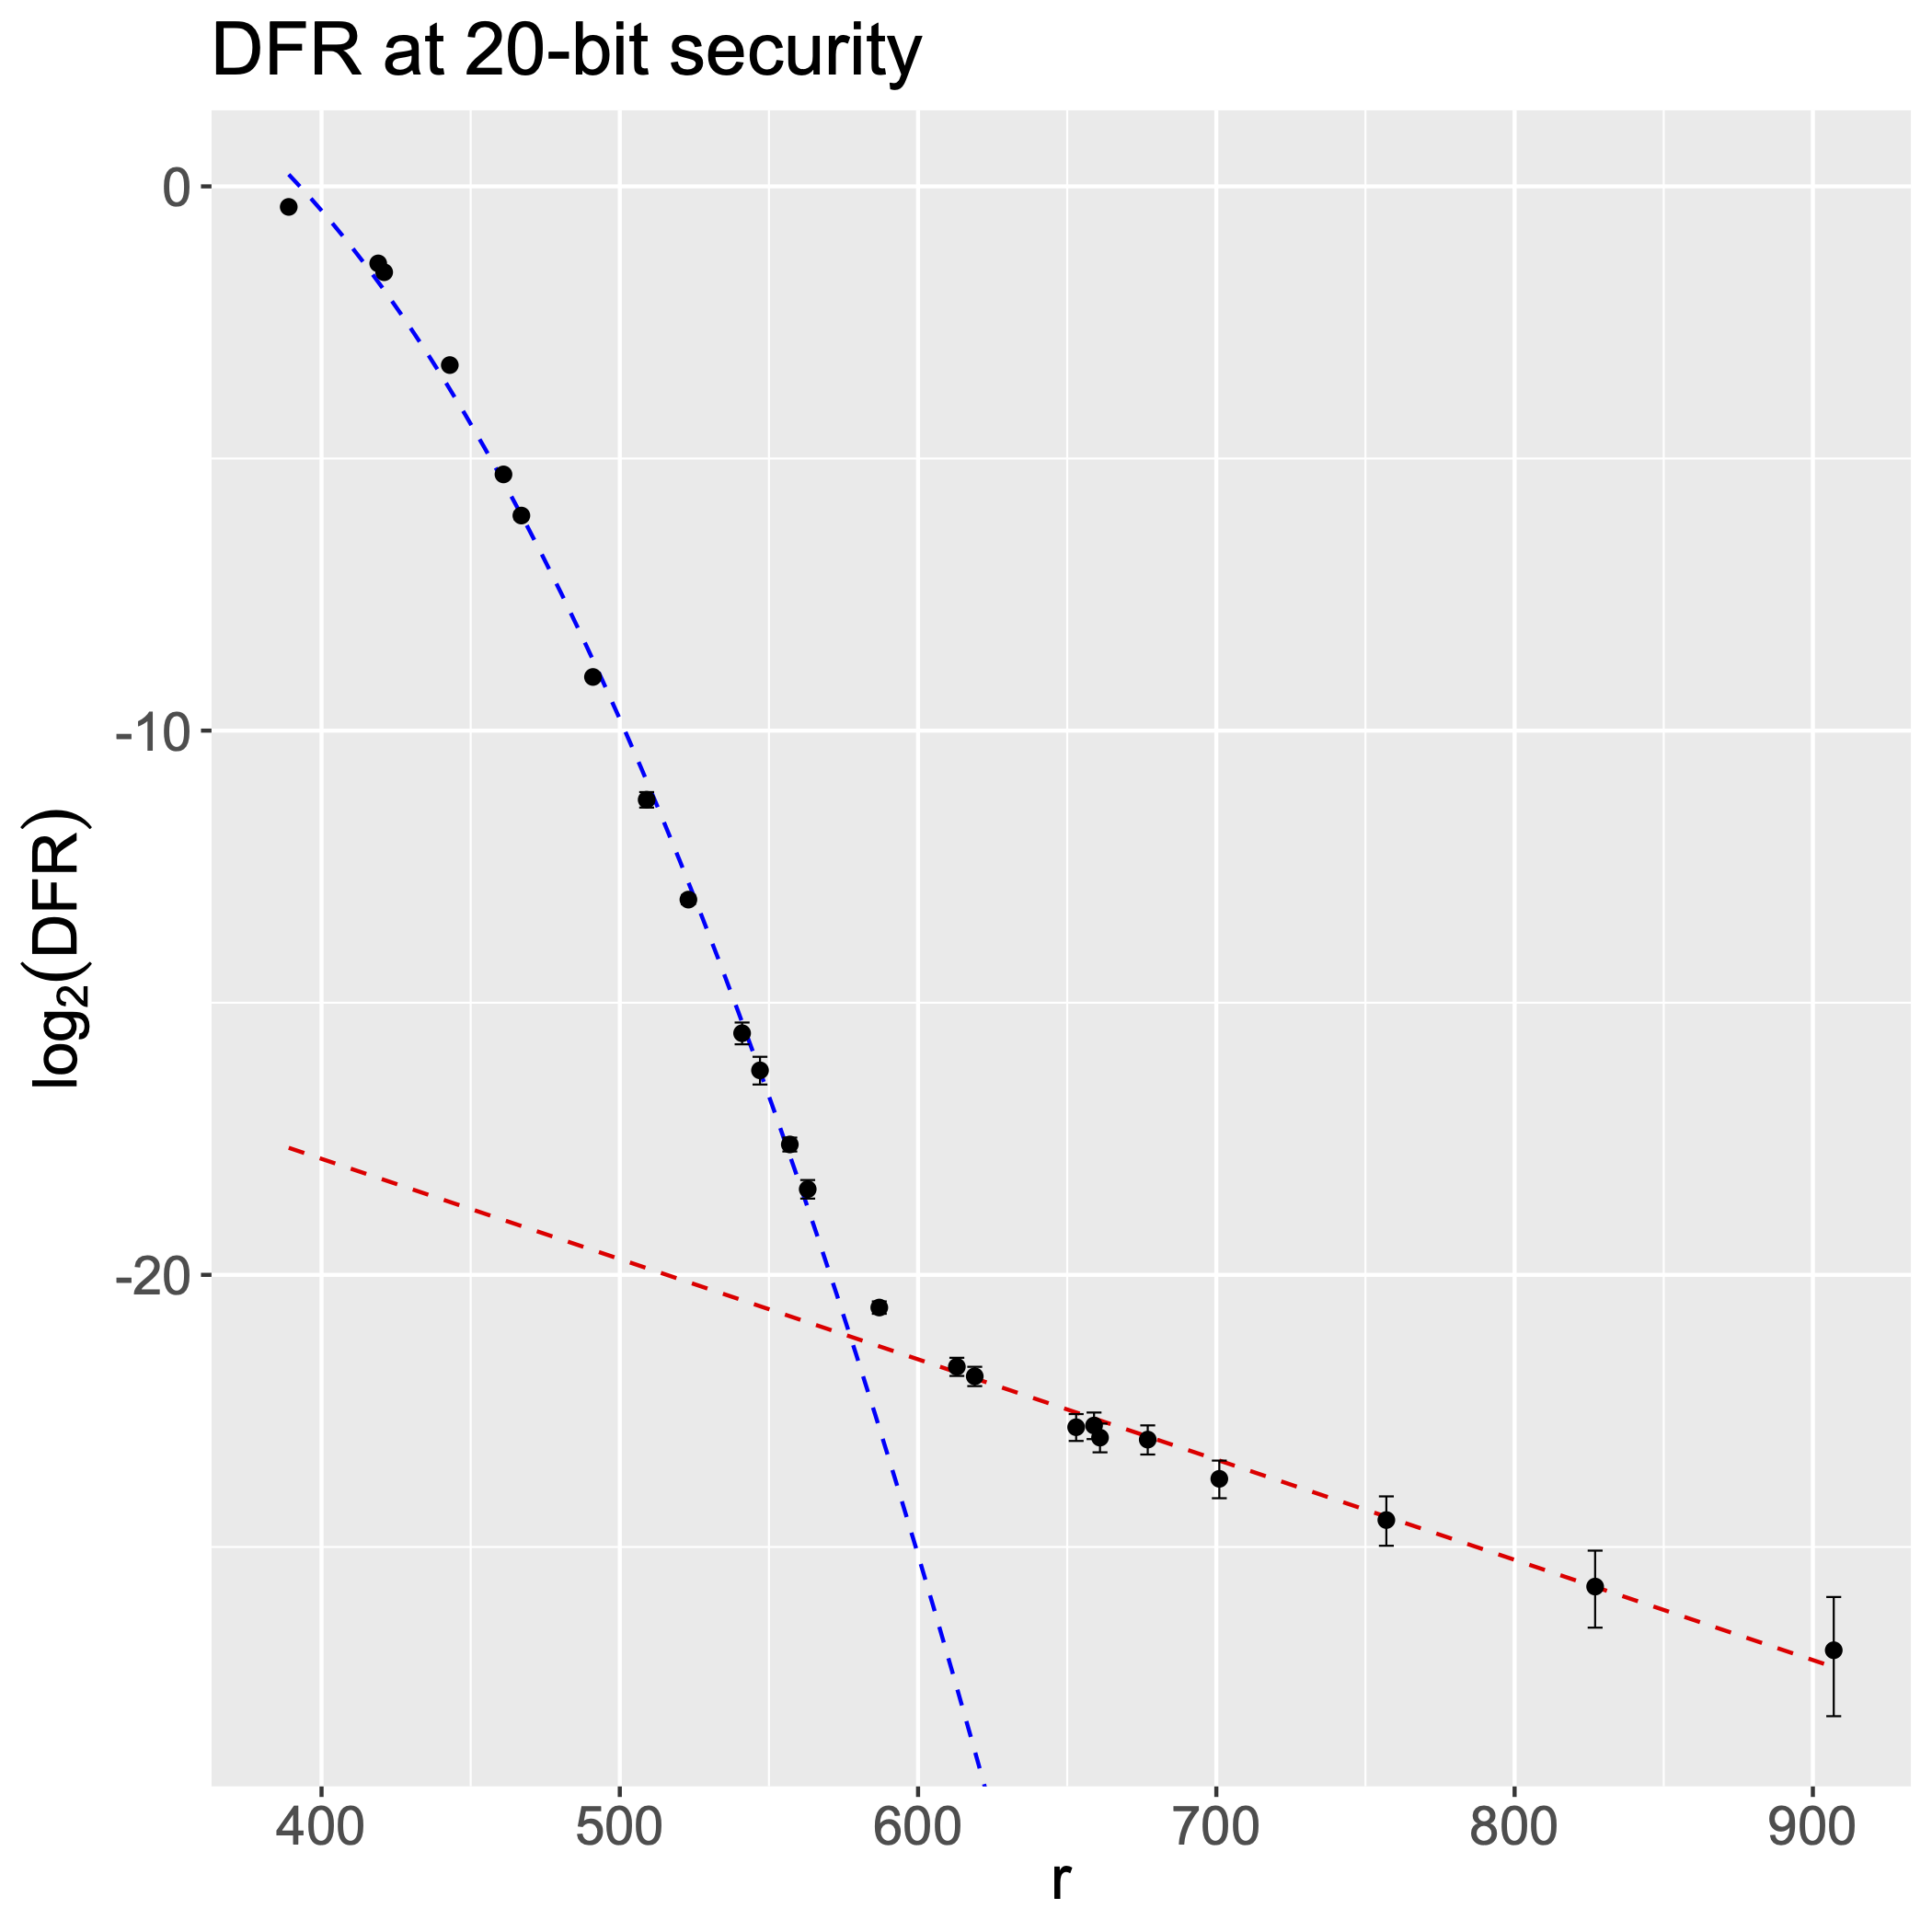
\includegraphics[width=0.49\textwidth]{2_bike/DFR-plot-T3.png}
    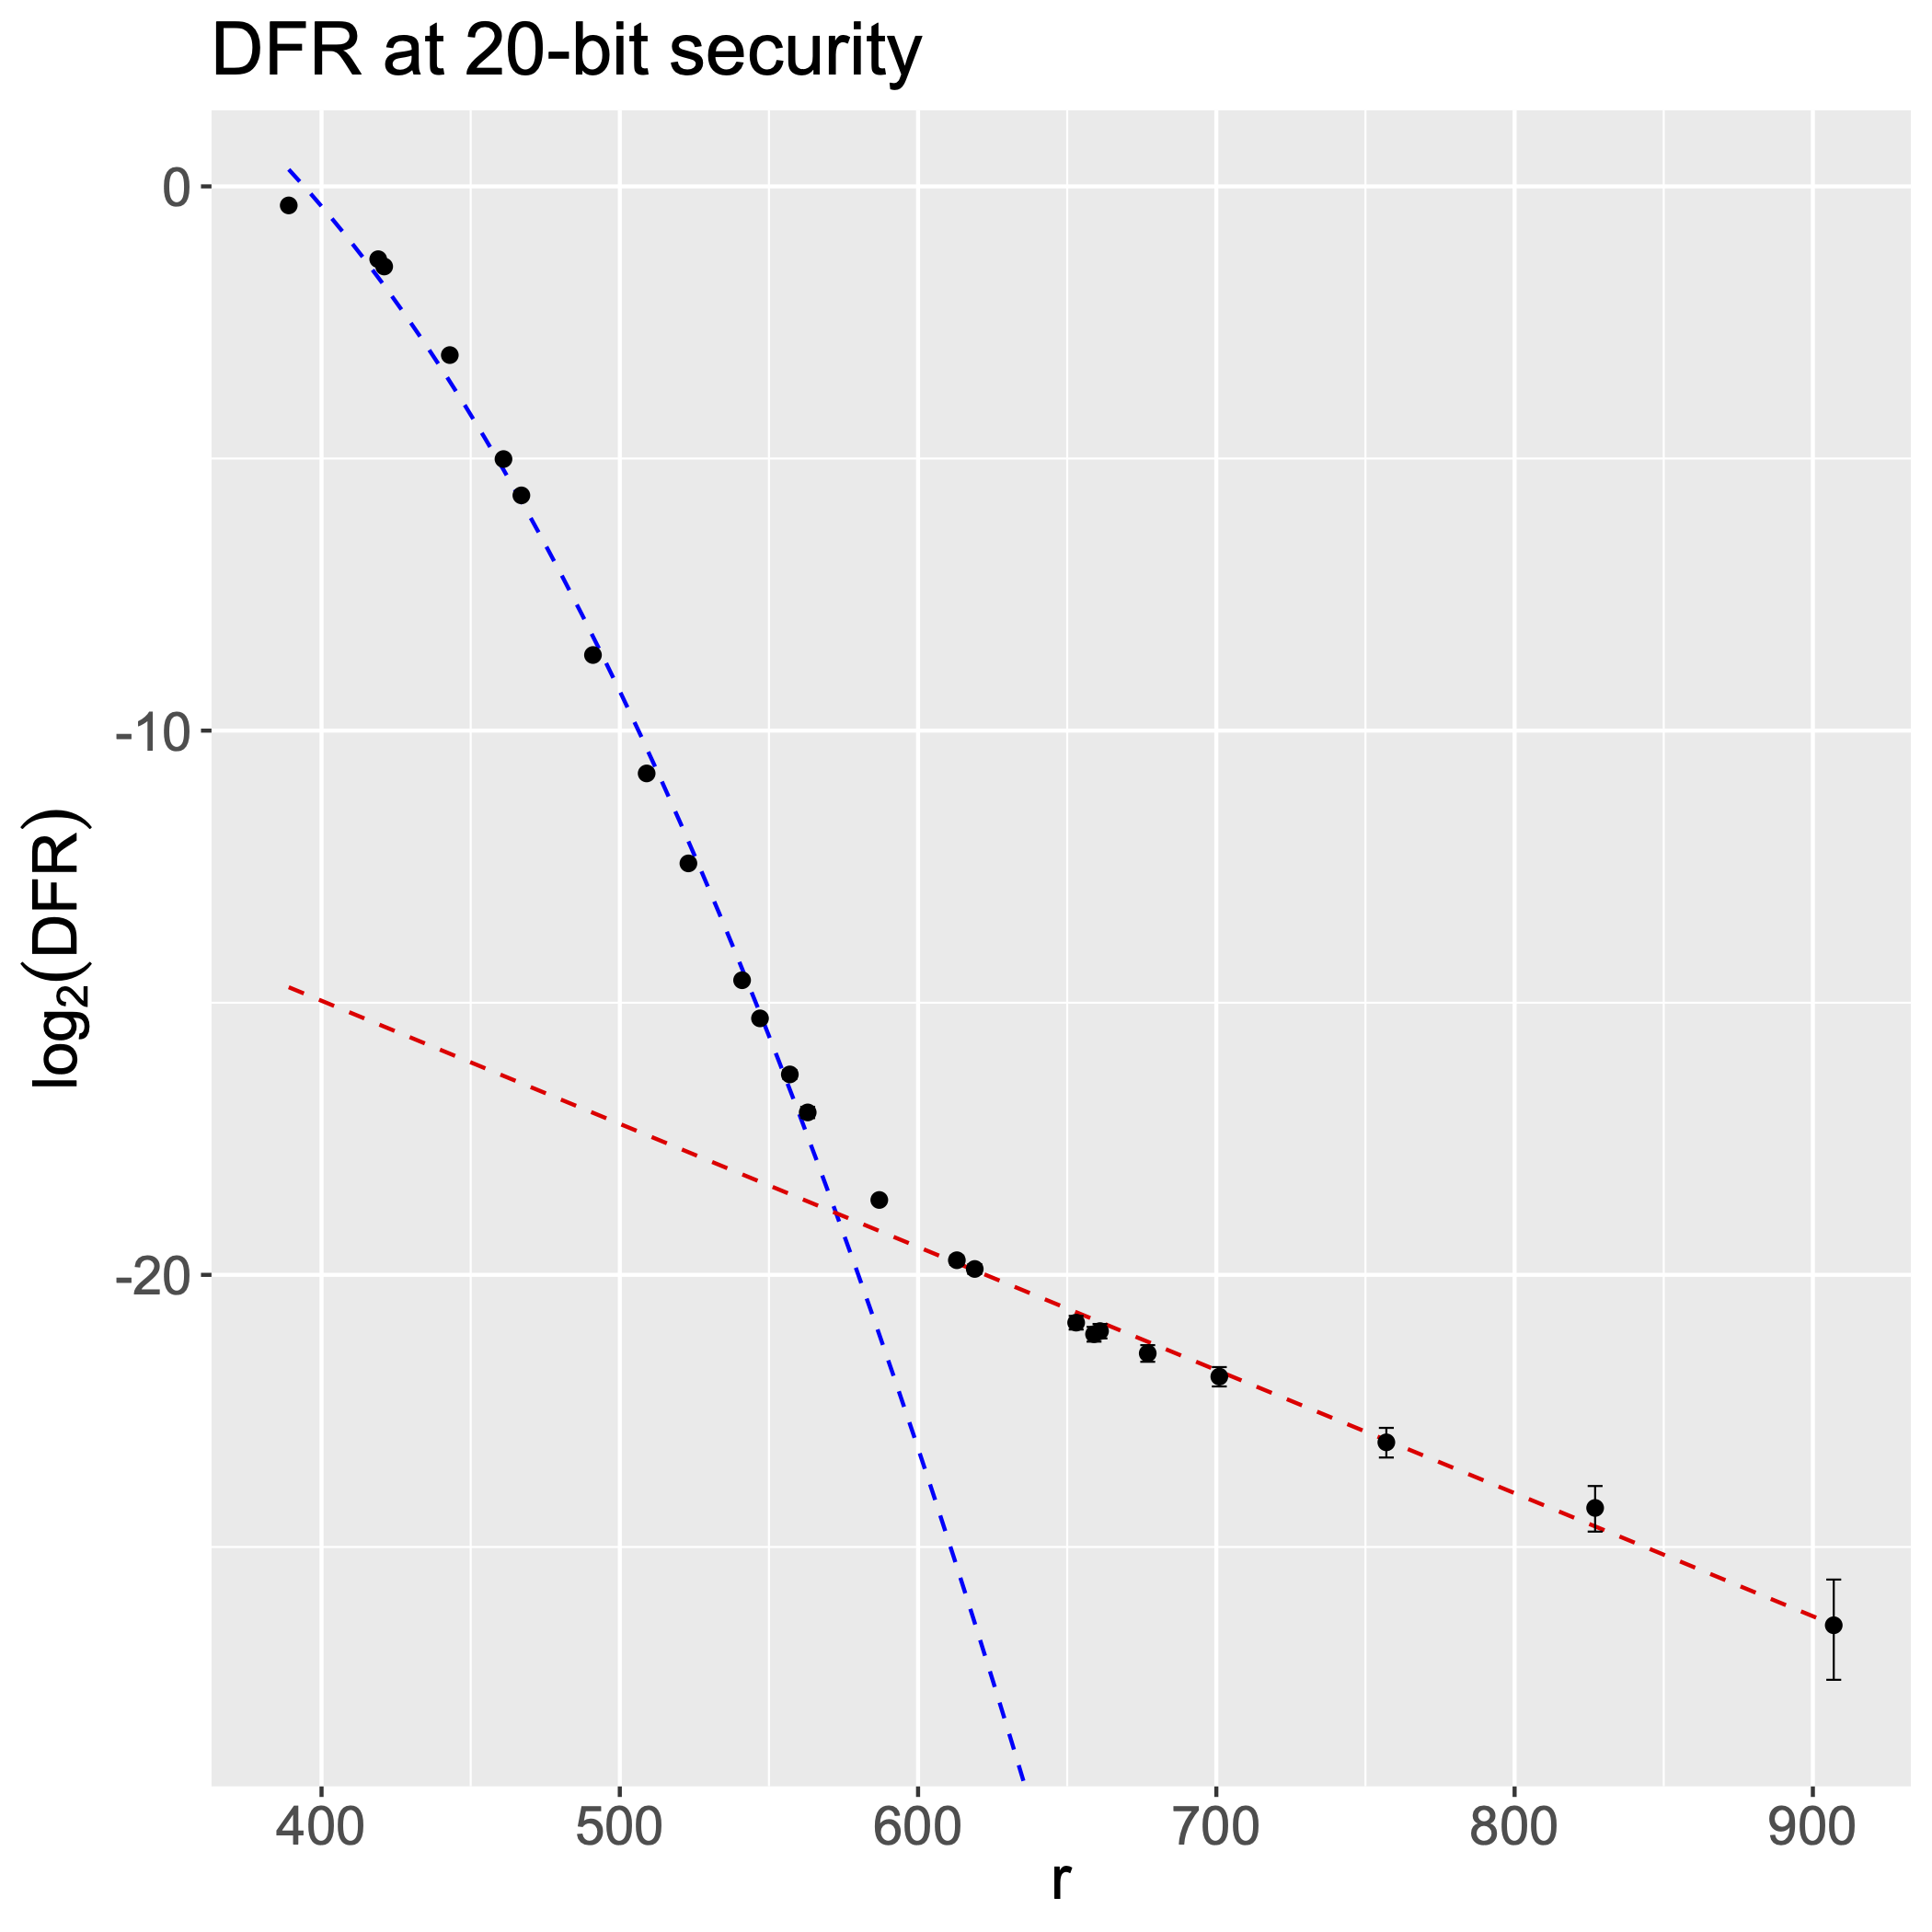
\includegraphics[width=0.49\textwidth]{2_bike/DFR-plot-random.png}
  \end{center}
  \caption{Semi-log plot of decoding failure rates for non-weak keys ($T = 3$, left) and for unfiltered random keys (right), with a 95\% confidence interval for each $r$. There is a quadratic best fit (blue) in the waterfall region and a linear best fit (red) in the error floor region ($r \geq 587$).}
  \label{fig:DFR}
\end{figure}

\newpage

\todo{Updated data available}
\begin{flushleft}
    \textbf{Table 6.1}: Decoding failure rates for $r$-values such that $389 \leq r \leq 827$, $r$ is prime, and $x^r - 1$ has only two irreducible factors modulo $2$. The data was computed using the parameters and methods described above.
    \end{flushleft}
\begin{table}[htb]
    \begin{center}
        \begin{tabular}{c|c|c|r}
            \;\;\;$r$\;\;\; & \;Decoding failures\;  & \;Decoding trials\;  & \;$\log_2(\mathrm{DFR})$ \\
            \hline
            389 & 939 & $10^3$ & $-0.09$ \\
            419 & 680 & $10^3$ & $-0.56$ \\
            421 & 652 & $10^3$ & $-0.62$ \\
            443 & 3289 & $10^4$ & $-1.60$ \\
            461 & 1172 & $10^4$ & $-3.09$ \\
            467 & 850 & $10^4$ & $-3.56$ \\
            491 & 1524 & $10^5$ & $-6.04$ \\
            509 & 380 & $10^5$ & $-8.04$ \\
            523 & 946 & $10^6$ & $-10.05$ \\
            541 & 164 & $10^6$ & $-12.57$ \\
            547 & 70 & $10^6$ & $-13.80$ \\
            557 & 177 & $10^7$ & $-15.79$ \\
            563 & 108 & $10^7$ & $-16.50$ \\
            587 & 128 & $10^8$ & $-19.58$ \\
            613 & 61 & $10^8$ & $-20.64$ \\
            619 & 60 & $10^8$ & $-20.67$ \\
            653 & 37 & $10^8$ & $-21.37$ \\
            659 & 35 & $10^8$ & $-21.45$ \\
            661 & 37 & $10^8$ & $-21.37$ \\
            677 & 24 & $10^8$ & $-21.99$ \\
            701 & 20 & $10^8$ & $-22.25$ \\
            757 & 8 & $10^8$ & $-23.58$ \\
            827 & 7 & $10^8$ & $-23.77$
        \end{tabular}
    \end{center}
    \label{table:DFR}
\end{table}

\section{DFR on $\mathcal{A}_{t,\ell}(\mathcal{S})$}

Recall that Vasseur identified three problematic sets of $(u,v)$-near codewords and proposed a study on the effect of proximity of error vectors to these sets by defining the set: $$\mathcal{A}_{t,\ell}(\mathcal{S}) := \{v \in \FF_2^{2r} : |v \star c| = \ell \text{ for some } c \in \mathcal{S} \}$$.

While $\ell$ measures the number of common intersections of an error vector with an element of $\mathcal{S}$, we can define another quantity that measures the distance of an error vector from $\mathcal{S}$:

\[
\delta(e) = |c| + t - 2\ell
\]

where $c\in \mathcal{S}$ is the vector with $|e \star c| = \ell$.

For $\ell$ high ( equivalently, $\delta$ low), decoding failures are extremely prevalent ( see Figure \ref{fig:DFR_CN2N}).

\begin{figure}[h]
    \centering
    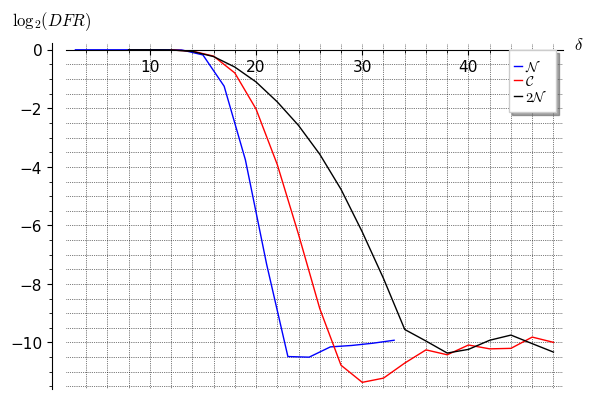
\includegraphics[scale=.75]{2_bike/DFR_20bit_CN2N_new.png}
    \caption{20-bit security DFR versus $\delta$ for near-codeword sets  $\mathcal{C},\mathcal{N}, 2\mathcal{N}$ for $r = 523$}
    \label{fig:DFR_CN2N}
\end{figure}

We study the relationship between $\mathcal{A}_{t,\ell}(\mathcal{S})$ for some $\ell$, $\mathcal{S} \in \{ \mathcal{C}, \mathcal{N}, 2\mathcal{N} \}$ and decoding failures. Our data shows that it is highly unlikely for a decoding failure vector to have a high intersection with an element in $\mathcal{S}$. For a vector $v$, we define the maximum overlap of $v$ for a fixed $\mathcal{S}$ by computing the largest $\ell$ such that $v \in \mathcal{A}_{t,\ell}(\mathcal{S})$. Using the experimental data from $r=587, N=10^9$ we recorded 557 total decoding failures and stored the 557 random error vectors that led to decoding failure. The relationship between these decoding failure vectors and the sets $\mathcal{S} $ is shown below:


\begin{figure}[htbp]
  \begin{center}
    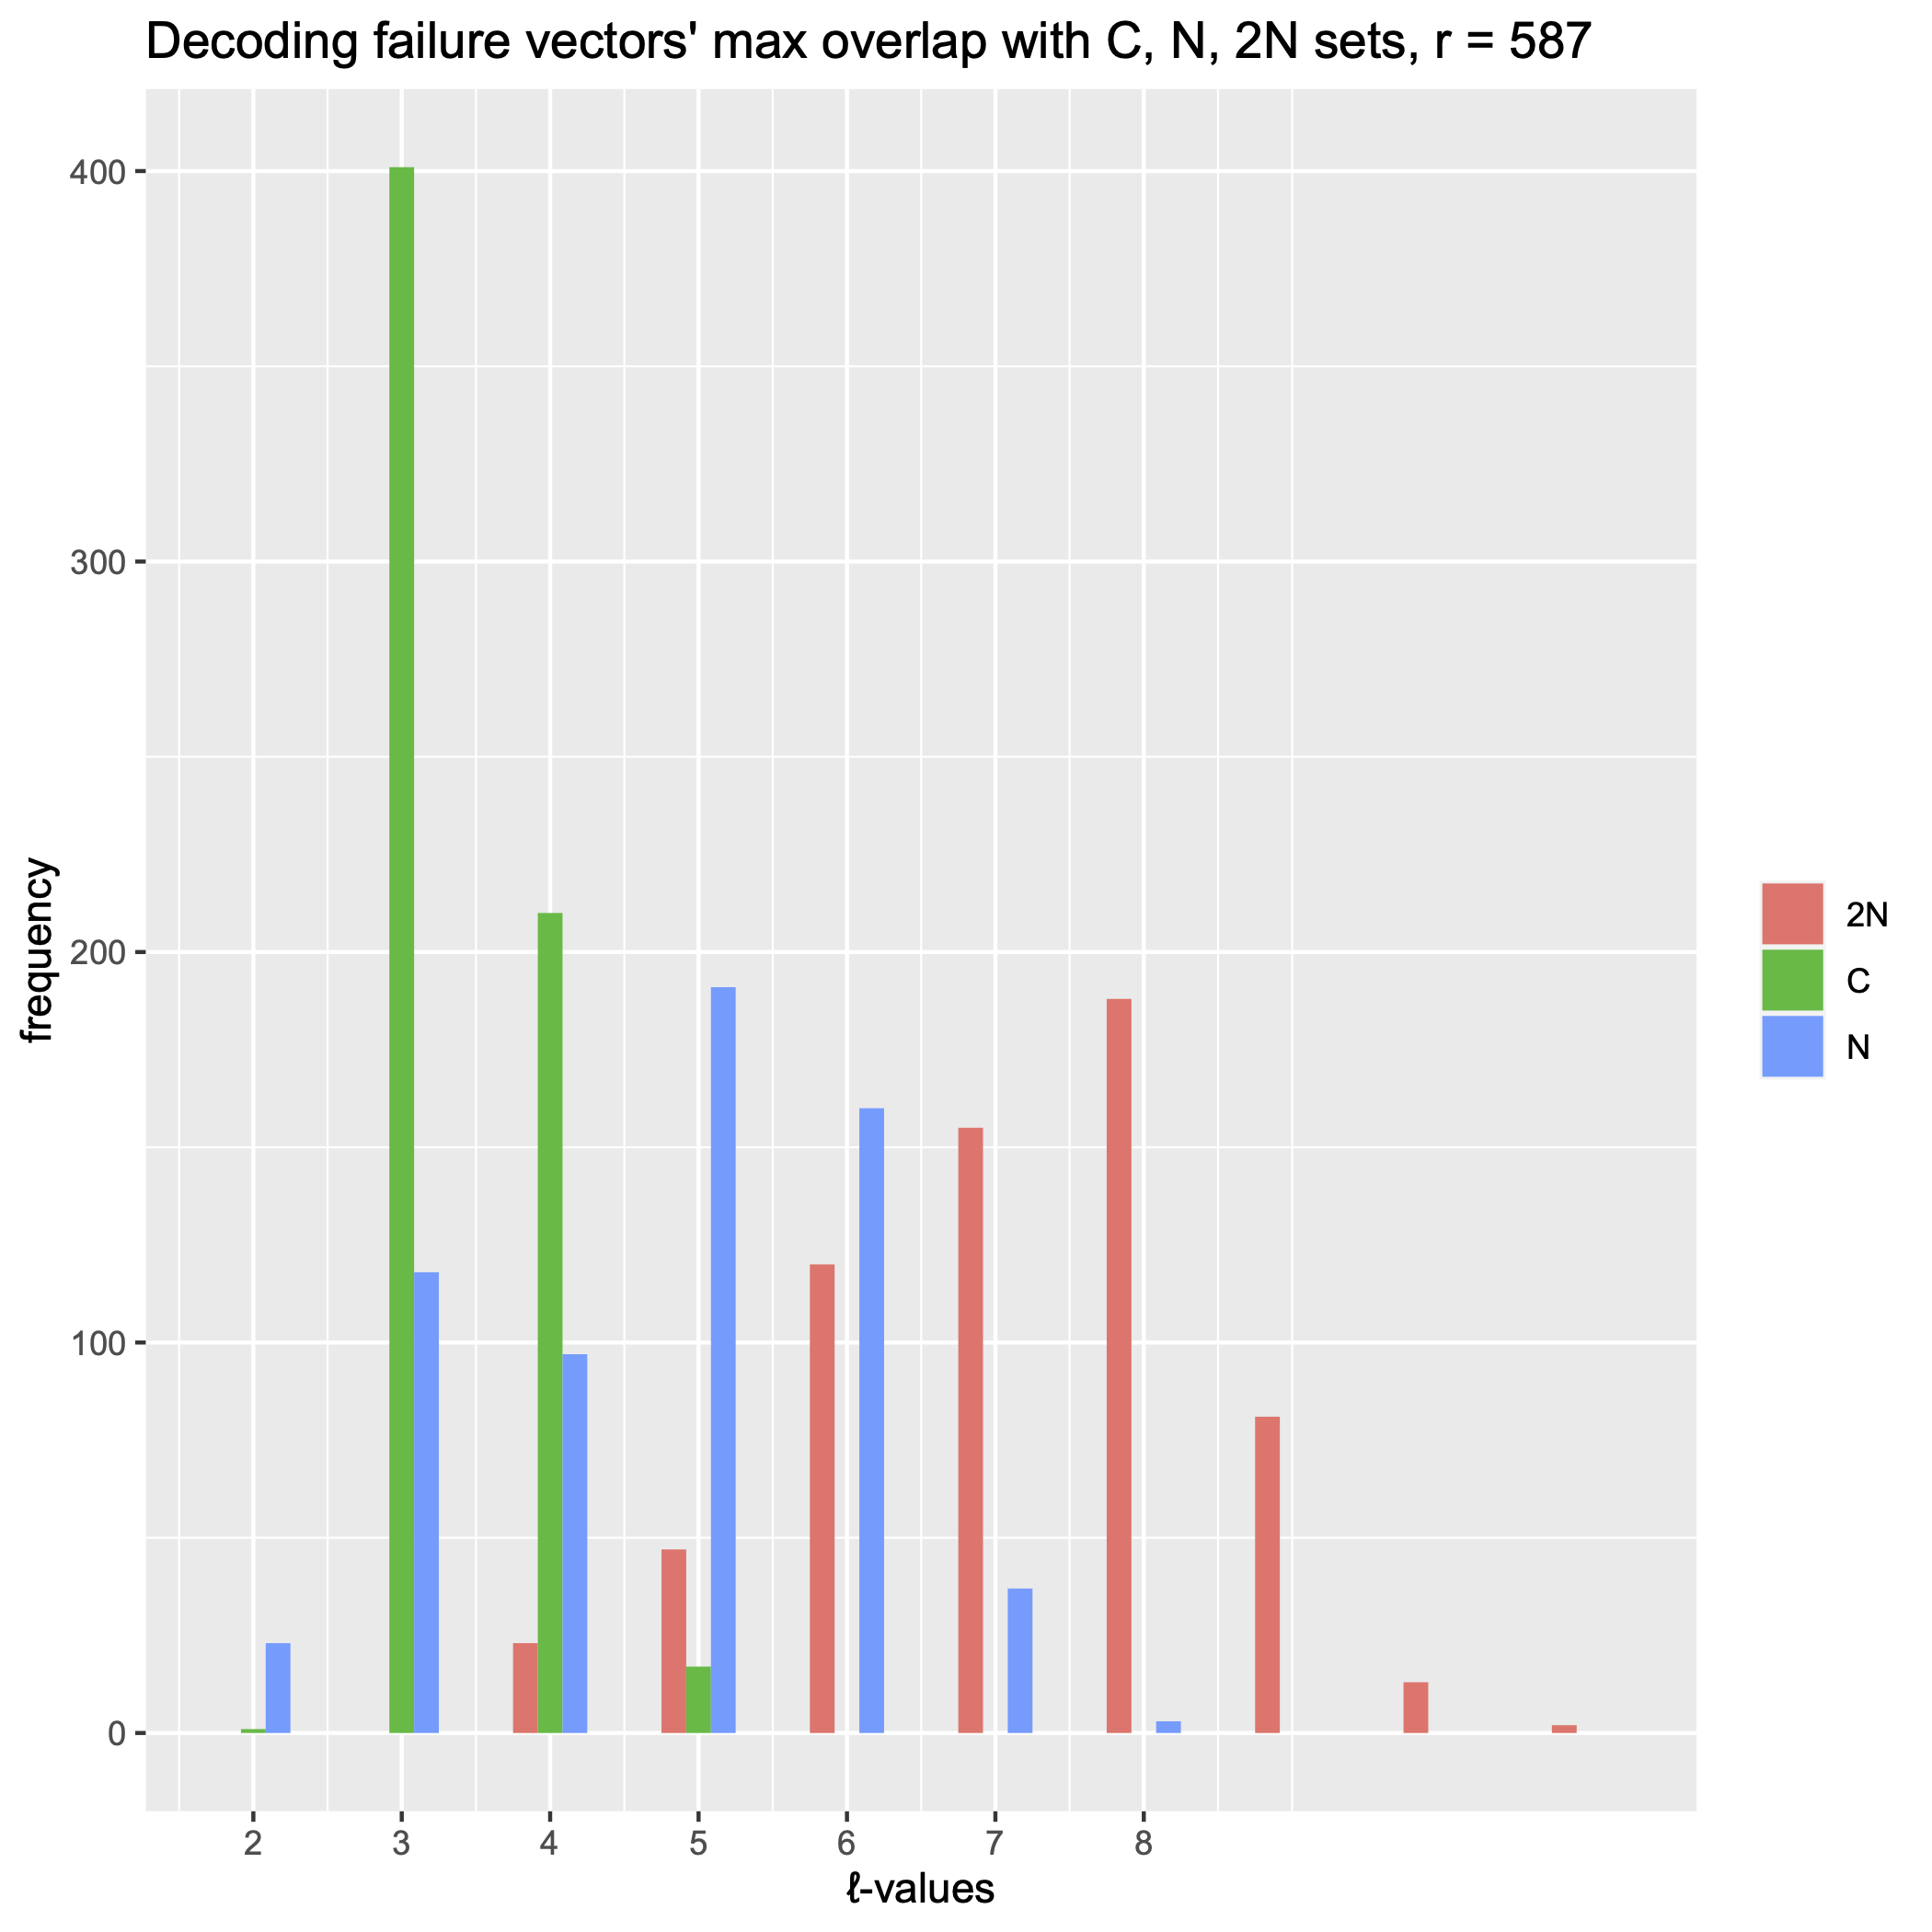
\includegraphics[width=0.49\textwidth]{2_bike/Rplot-587-df.png}
    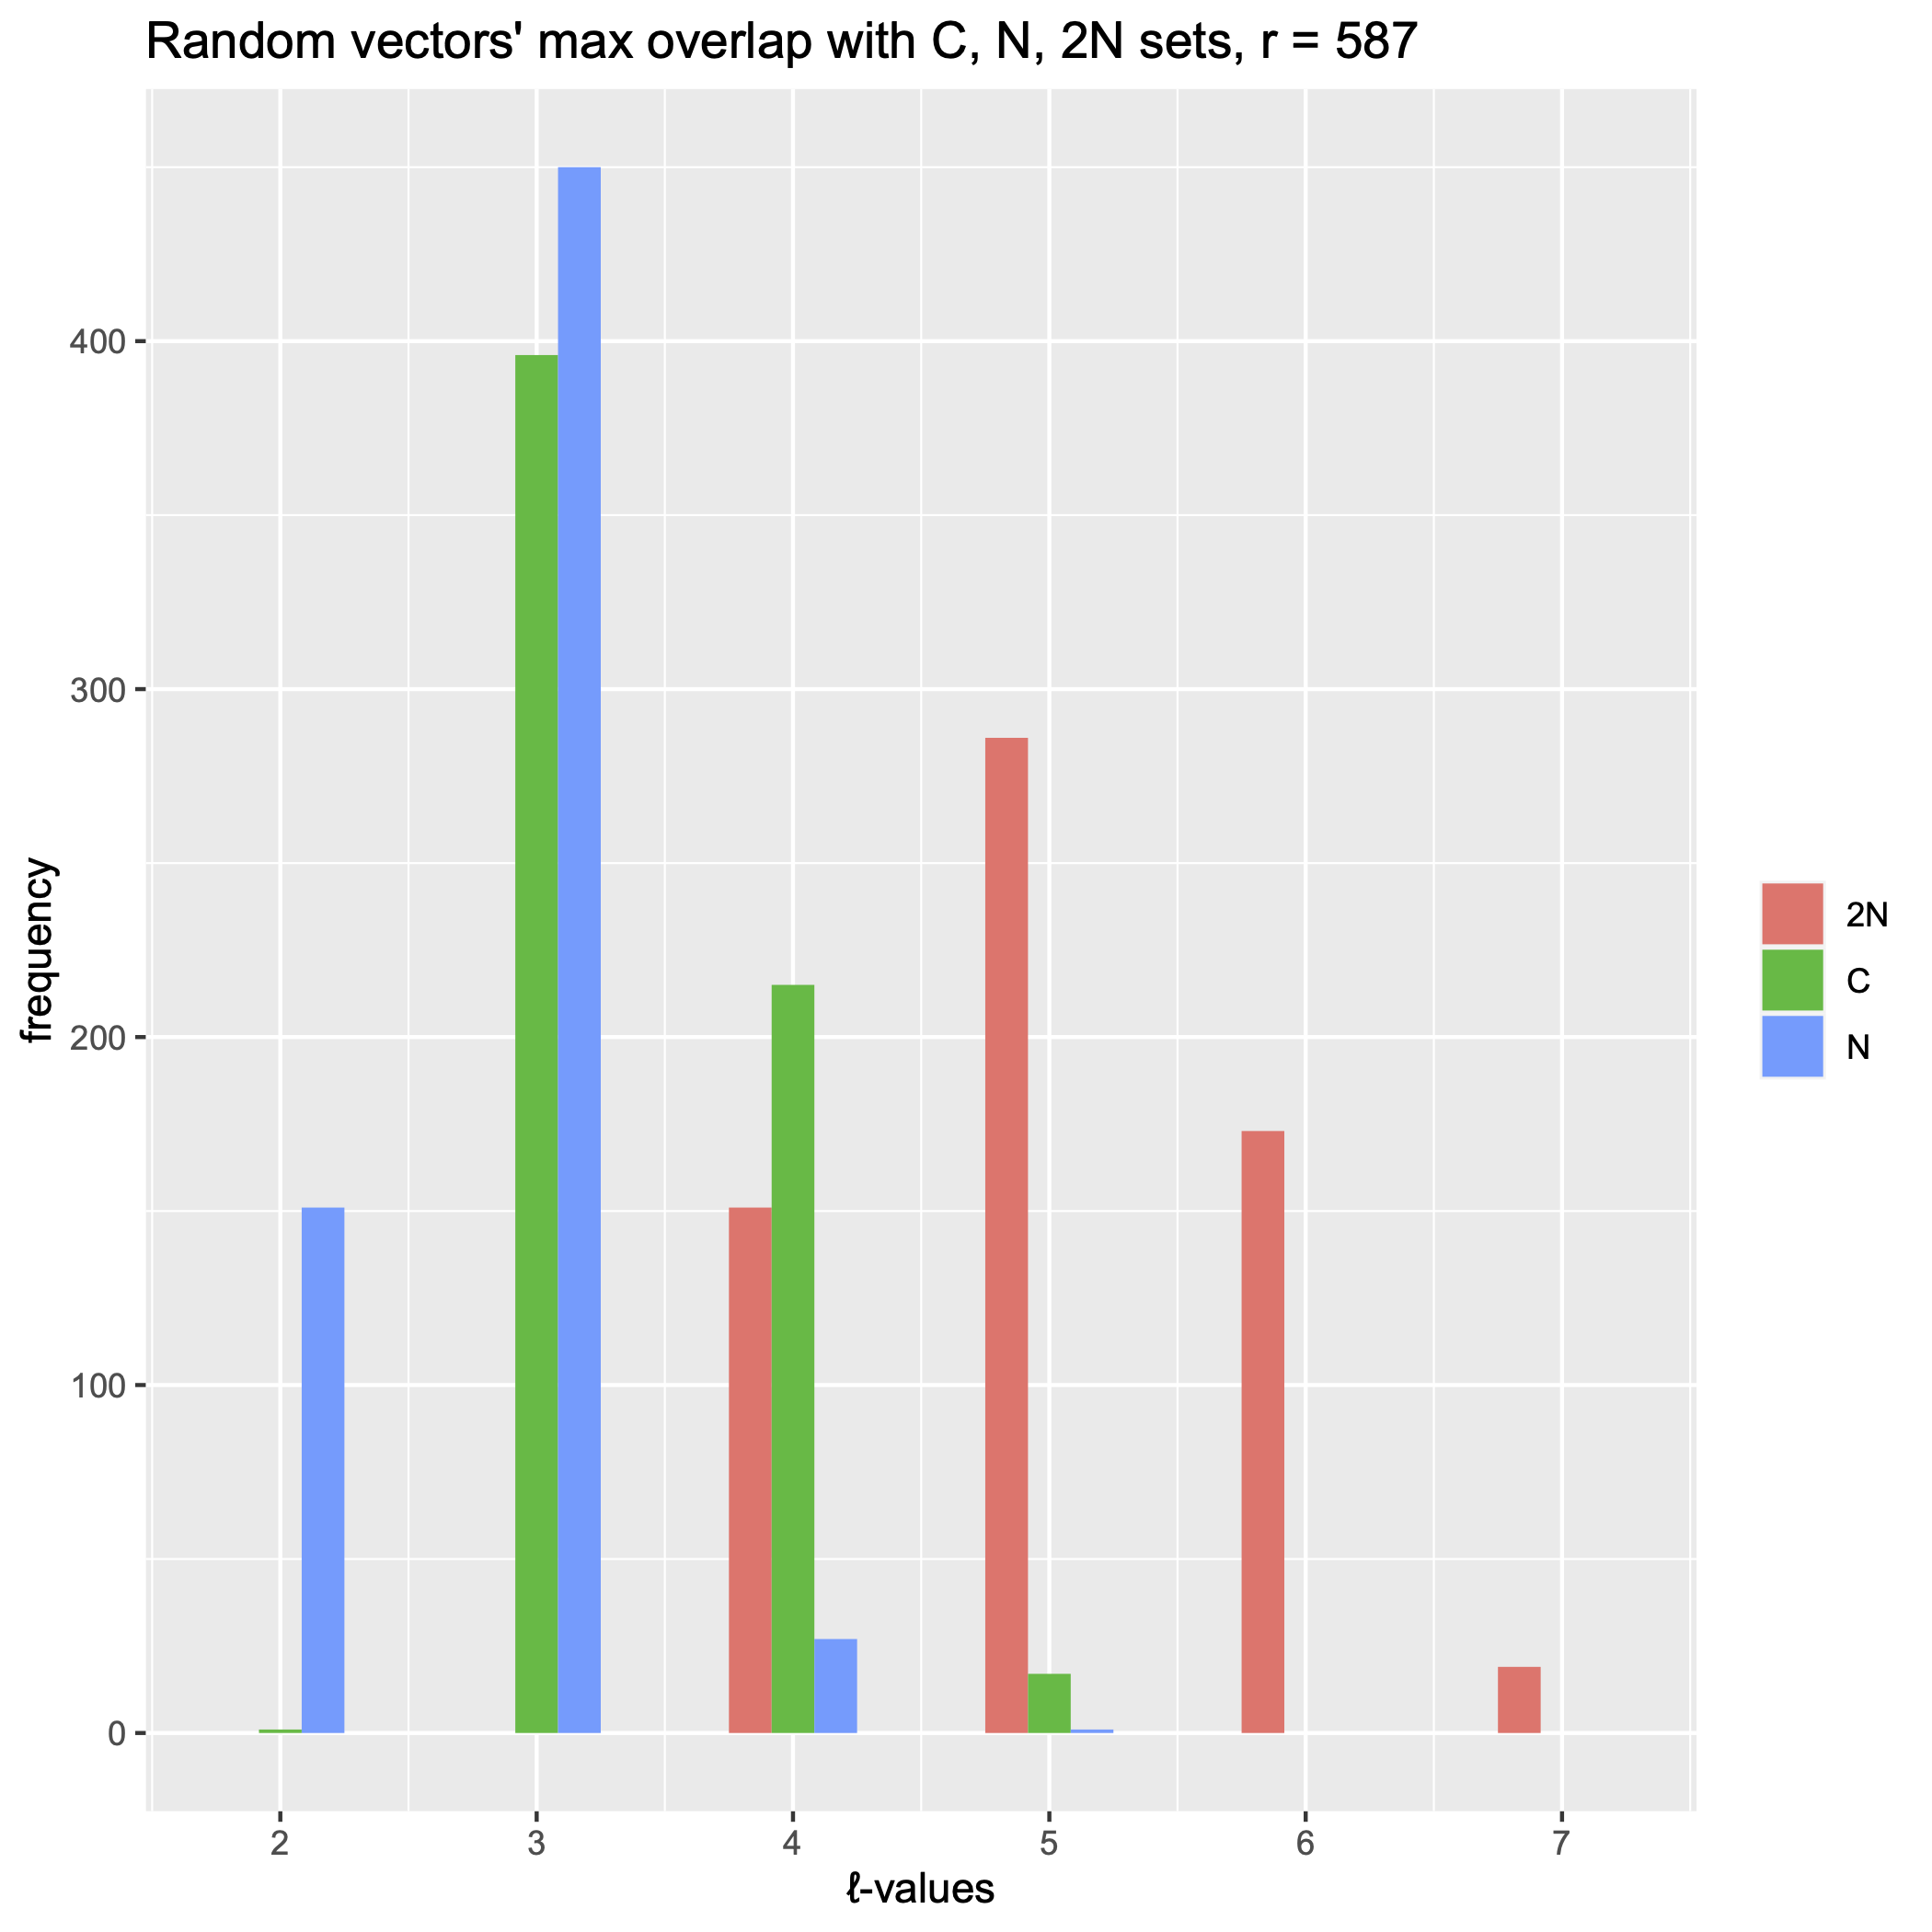
\includegraphics[width=0.49\textwidth]{2_bike/Rplot-587-random.png}
  \end{center}
  \caption{Distribution of maximum overlaps of decoding failure vectors (left) or random vectors (right) with the sets $\mathcal{C}$, $\mathcal{N}$, and $2\mathcal{N}$ for $r = 587$, using a weak key threshold of $T = 3$ to generate keys.}
  \label{fig:AtlS}
\end{figure}

The cases where $\ell > 10$ are rare. It is expected that these problematic sets contribute to the decoding failures occuring in error floor region and our data suggests that some proportion of decoding failures can be explained by their proximity to $\mathcal{N}$ or $2\mathcal{N}$. However, it is also the case that a significant of the errors causing decoding failures do not have more overlap with $\mathcal{S}$ than typical random vectors. Further analysis is needed to determine what proportion of decoding failures are explained by this proximity.
\section{Syndrome weight as an indicator}

From the previous analysis of $\mathcal{A}_{t,\ell}(\mathcal{S})$, the syndrome weights of error vectors causing decoding failures in those sets are low. It is natural to investigate to if the syndrome weight can serve as a predictor for decoding failures. 

For the experiment, for each suitable $r$, we generate $10^3$ instances of non-weak parity check matrices $\mathbf{H}$, random error vectors $e$, and then we compute the average weight of their syndromes $s=He^T$. For decoding failure error vectors, we extract the information from our previous DFR simulations to get the nonweak parity check matrices and the corresponding vector causing decoding failures, and then we compute the average weight of their syndromes. Figure \ref{fig:syndrome-weights} below gives a summary of our results:

\begin{figure}[htbp]
  \begin{center}
    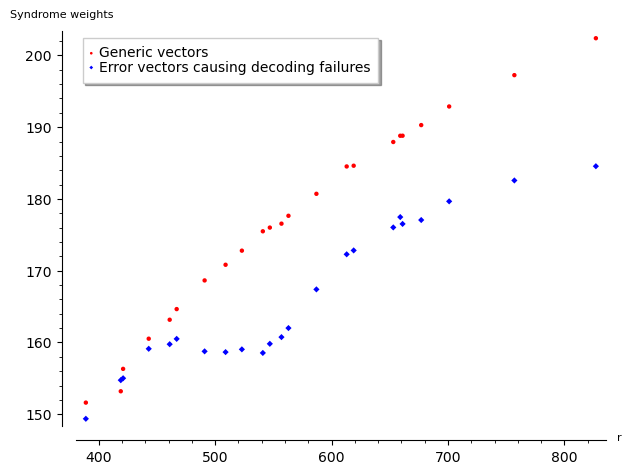
\includegraphics[width=0.49\textwidth]{2_bike/average_sw_generic_vs_DF_T3.png}
    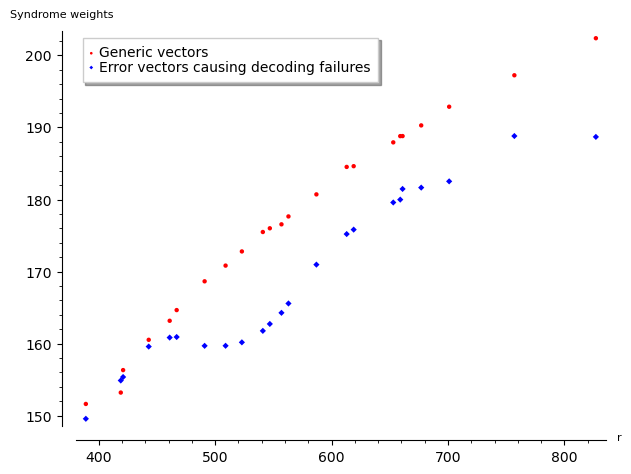
\includegraphics[width=0.49\textwidth]{2_bike/average_sw_generic_vs_DF_random.png}
  \end{center}
  \caption{Distribution of syndrome weights for random error vectors (red) versus error vectors causing decoding failures (blue). The left plot is for non-weak keys (with threshold $T = 3$); the right plot is for unfiltered random keys.}
  \label{fig:syndrome-weights}
\end{figure}

The simulations suggest that syndrome weights of generic vectors tend to follow a normal distribution while the error vectors causing decoding failures have syndrome weights that are more concentrated around the mean, which we hypothesise to be lower than that of the generic vectors; see Figure \ref{fig:r87_comparison} for the case $r=587$, where we compare the syndrome weights of the \todo{check} 128 vectors which caused decoding failures with the syndrome weights of the $10^5$ randomly generated vectors of the same weight $t = 18$.

\todo{might need to generate r587df again}
\begin{figure}[ht]
\centering
\begin{subfigure}[b]{.45\textwidth}
  \centering
  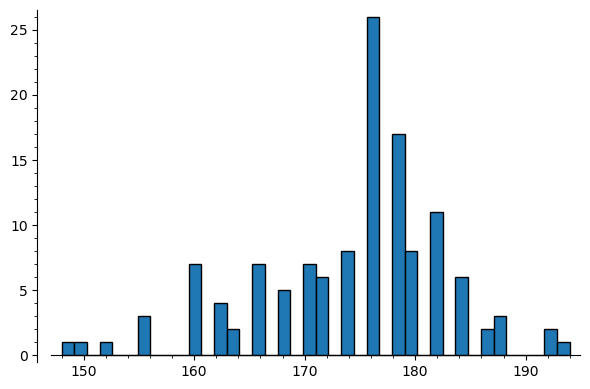
\includegraphics[scale=.45]{2_bike/r587df.png}
  \caption{Decoding failure vectors}
  \label{fig:r587df}
\end{subfigure}
\begin{subfigure}[b]{.45\textwidth}
  \centering
  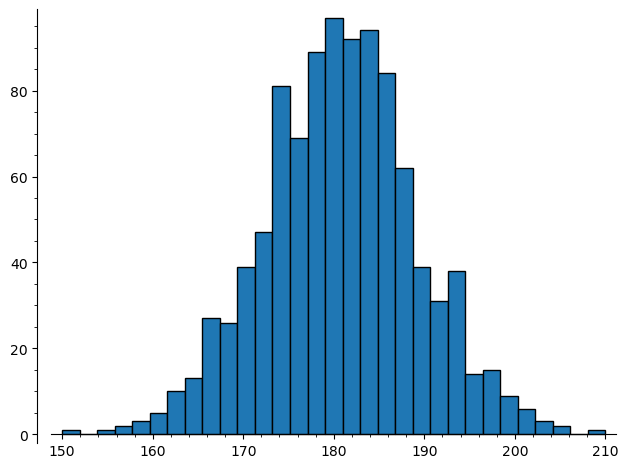
\includegraphics[scale=.45]{2_bike/r587g_new.png}
  \caption{Randomly generated vectors}
  \label{fig:r587g}
\end{subfigure}
\caption{A comparison of syndrome weights for $r = 587$ between the 128 error vectors which were found to be involved in decoding failures and $10^5$ random vectors. Vertical axis is frequency, and horizontal axis is syndrome weight.}
\label{fig:r87_comparison}
\end{figure}

Using this data, we explore whether or not there is convincing evidence that the syndrome weights of error vectors causing decoding failures are lower than those of generic vectors. The null hypothesis is that there is no difference between the two groups in consideration while the alternative hypothesis is that the generic vectors have higher syndrome weights. Both data come from random, independent sampling and have data sets with more than 30 observations. The difference in sample means may be modeled using a $t$-distribution. For each $r$, one could compute the point estimates $m_{\text{generic}} - m_{\text{DF}}$ of population difference $\mu = \mu_{\text{generic}} - \mu_{\text{DF}}$ and standard errors of the point estimate 

$$SE = \sqrt{\frac{\sigma_{\text{generic}}^2}{N_{\text{generic}} } +\frac{\sigma_{\text{DF}}^2}{N_{\text{DF}} } }.$$

With this information, one could compute the test statistic for this (one-tailed) test by the formula $T = \frac{\mu - 0}{SE}$. Using either a $t$-table or statistics software, we can find appropriate degrees of freedom and from there, the $p$-value, for each $r$. Our conclusion is that for the sixteen $r$-values in the range $509 \leq r \leq 827$, the $p$-value is less than the significance value $\alpha = 0.01$, and therefore we reject the null hypothesis, i.e., syndrome weights of error vectors causing decoding failures are lower than those of generic vectors.

A general summary of the test statistic values $m_{\text{generic}} - m_{\text{DF}}$ and the corresponding $p$-values can be found in Table~\ref{table:hyp_test_ts_and_ps}.\todo{check calculations}

\begin{table}[ht]
\centering
\begin{tabular}{c|c|c}
$r$   & $m_{\text{generic}} - m_{\text{DF}}$ & $p$                \\
\hline
509 & 9.29                          & $< 0.00001$ \\
523 & 8.60                          & $< 0.00001$ \\
541 & 9.79                          & $< 0.00001$ \\
547 & 9.29                          & $< 0.00001$ \\
557 & 6.20                          & $< 0.00001$ \\
563 & 8.61                          & $< 0.00001$ \\
587 & 6.56                          & $< 0.00001$ \\
613 & 10.92                         & $< 0.00001$ \\
619 & 8.86                          & $< 0.00001$ \\
653 & 15.99                          & $< 0.00001$ \\
659 & 11.49                          & $< 0.00001$ \\
661 & 9.40                          & $< 0.00001$ \\
677 & 14.45                          & $< 0.00001$ \\
701 & 17.58                          & $< 0.00001$ \\
757 & 16.25                          & $ 0.00278$ \\
827 & 17.53                          & $ 0.00002$ \\

\end{tabular}
\caption{Hypothesis test results for $509 \leq r \leq 827$, with the corresponding test statistic values and $p$-values, indicating the vectors causing decoding failures do have lower syndrome weights than generic vectors for $509 \leq r \leq 701$, notably a selection of $r$-values where the waterfall region meets the error floor in the DFR graph of Figure~\ref{fig:DFR}.}\label{table:hyp_test_ts_and_ps}
\end{table}




\section{Conclusion and future work}

In the analysis of the BIKE cryptosystem at the $20$-bit security level, we have reproduced the error floor phenomenon and obtained large amount of data for analysis. We found that decoding failure error vectors have lower syndrome weights than those of random vectors. Furthermore, as identified in \cite{Vasseur-thesis,Vasseur:2021:eprint}, the three classes of problematic error vectors $\mathcal{C}, \mathcal{N}, 2\mathcal{N}$ and their proximity sets $\mathcal{A}_{t,\ell}(\mathcal{S})$ contain many elements that cause decoding failures. However, our experiments showed these sets are not responsible the bulk of decoding failures.

It therefore remains to further identify classes of error vectors causing decoding failures in our experiments. As part of an ongoing work, the small parameters allow us to adopt a graph theoretic approach to study the Tanner graph representations of these QC-MDPC codes, which allow us to study interesting behaviours coming from absorbing and trapping sets.



%% END MATTER
% \printindex %% Uncomment to display the index
% \nocite{}  %% Put any references that you want to include in the bib 
%               but haven't cited in the braces.
\bibliographystyle{alpha}  %% This is just my personal favorite style. 
%                              There are many others.
%\setlength{\bibleftmargin}{0.25in}  % indent each item
%\setlength{\bibindent}{-\bibleftmargin}  % unindent the first line
%\def\baselinestretch{1.0}  % force single spacing
%\setlength{\bibitemsep}{0.16in}  % add extra space between items
\bibliography{template}  %% This looks for the bibliography in template.bib 
%                          which should be formatted as a bibtex file.
%                          and needs to be separately compiled into a bbl file.
\singlespace  %to force bibilography environment to use single spacing for each entry 
              %double spacing between entries remains
\end{document}

